\documentclass{beamer}
\input{../style/cours-style.sty}

% Title
\title[PYDATA]{Python - Data Scientist}
\author{Christophe Brun}
\institute{Digicomp}
\date{17 mai 2024}
\beamertemplatenavigationsymbolsempty

\titlegraphic{
    \bigbreak
    
\includegraphics[width=5cm]{image/digicomp-logo}
    \bigbreak
    Digital competence. Made of People.
    \bigbreak
}

\begin{document}

    \begin{frame}
        \titlepage
        \bigbreak
        \centering
        \url{https://github.com/DigicompClassesByPapIT/PYDATA}
    \end{frame}


    \section{Table des matières}\label{sec:toc}

    \begin{frame}{Table des matières}
        \begin{tiny}
            \begin{multicols}{3}
                \tableofcontents
            \end{multicols}
        \end{tiny}
    \end{frame}


    \section{Programme du module}\label{sec:programme-du-module}

    \begin{frame}{Python - Data Scientist}{Contenu des 2 jours}
        \begin{tiny}
            \begin{multicols}{3}
                \begin{itemize}
                {\tiny
                \item Programmation fonctionnelle
                    \begin{itemize}
                        \tiny
                        \item Expressions lambda
                        \item List comprehension
                    \end{itemize}

                    \item Jupyter Notebook
                    \begin{itemize}
                        \tiny
                        \item Fonctionnement local, serveur
                        \item Interface et commandes
                    \end{itemize}

                    \item NumPy
                    \begin{itemize}
                        \tiny
                        \item Création et manipulation de tableaux et matrices NumPy
                        \item Indexation et sélection
                        \item Manipulations arithmétiques, broadcasting
                        \item Fonctions statistiques
                    \end{itemize}

                    \item Pandas
                    \begin{itemize}
                        \tiny
                        \item Structures de données (Series, DataFrame, Panel)
                        \item Indexation et sélection
                        \item Fonctions statistiques
                        \item Combinaison des données (concat, append, merge, join)
                        \item Fenêtrage
                        \item Groupement et agrégation
                        \item Données temporelles
                    \end{itemize}

                    \item Chargement et sauvegarde des données
                    \begin{itemize}
                        \tiny
                        \item Traitement des principaux formats de fichiers
                        \begin{itemize}
                            \tiny
                            \item Excel, CSV, XML, JSON
                        \end{itemize}
                        \item Requêtes SQL avec Pandas
                    \end{itemize}

                    \item Préparation et nettoyage des données
                    \begin{itemize}
                        \tiny
                        \item Traitement des données manquantes
                        \item Combinaison et transformation de données
                        \item Agrégation et regroupement de données
                        \item Traitement des données temporelles
                    \end{itemize}

                    \item Visualisation avec Matplotlib, Seaborn et Plotly
                    \begin{itemize}
                        \tiny
                        \item Types de graphiques
                        \begin{itemize}
                            \tiny
                            \item Ligne, point, histogramme, bar, pie, \ldots{}
                        \end{itemize}
                        \item Label, légende, grille, axes, titre
                        \item Sauvegarde des graphiques
                        \item Visualisation avec Seaborn
                        \item Visualisation web interactive avec Plotly
                    \end{itemize}

                    \item Exemple d'analyse de données financières

                    \item Introduction au Machine Learning
                }
                \end{itemize}
            \end{multicols}
        \end{tiny}

    \end{frame}


    \section{Introduction}\label{sec:introduction}


    \begin{frame}{Formateur sur Linux}{Christophe Brun, conseil en développement informatique}

        \begin{columns}
            \column{0.7\textwidth}
            \begin{itemize}
                \item Développeur freelance (Python, Java, CoBOL) et data at scale.

                \item 7 ans de conseil en développement au sein d'SSII~.

                \item 8 ans de conseil en développement en indépendant, \href{https://papit.fr}{PapIT}.

                \item Passionné~!
                \bigbreak
                \begin{columns}
                    \column{0.5\textwidth}
                    \centering
                    
\includegraphics[width=3cm]{image/logo-uppa}
                    \column{0.5\textwidth}
                    \centering
                    
\includegraphics[width=3cm]{image/logo-universite-bordeaux}
                \end{columns}
            \end{itemize}
            \column{0.3\textwidth}
            \centering
            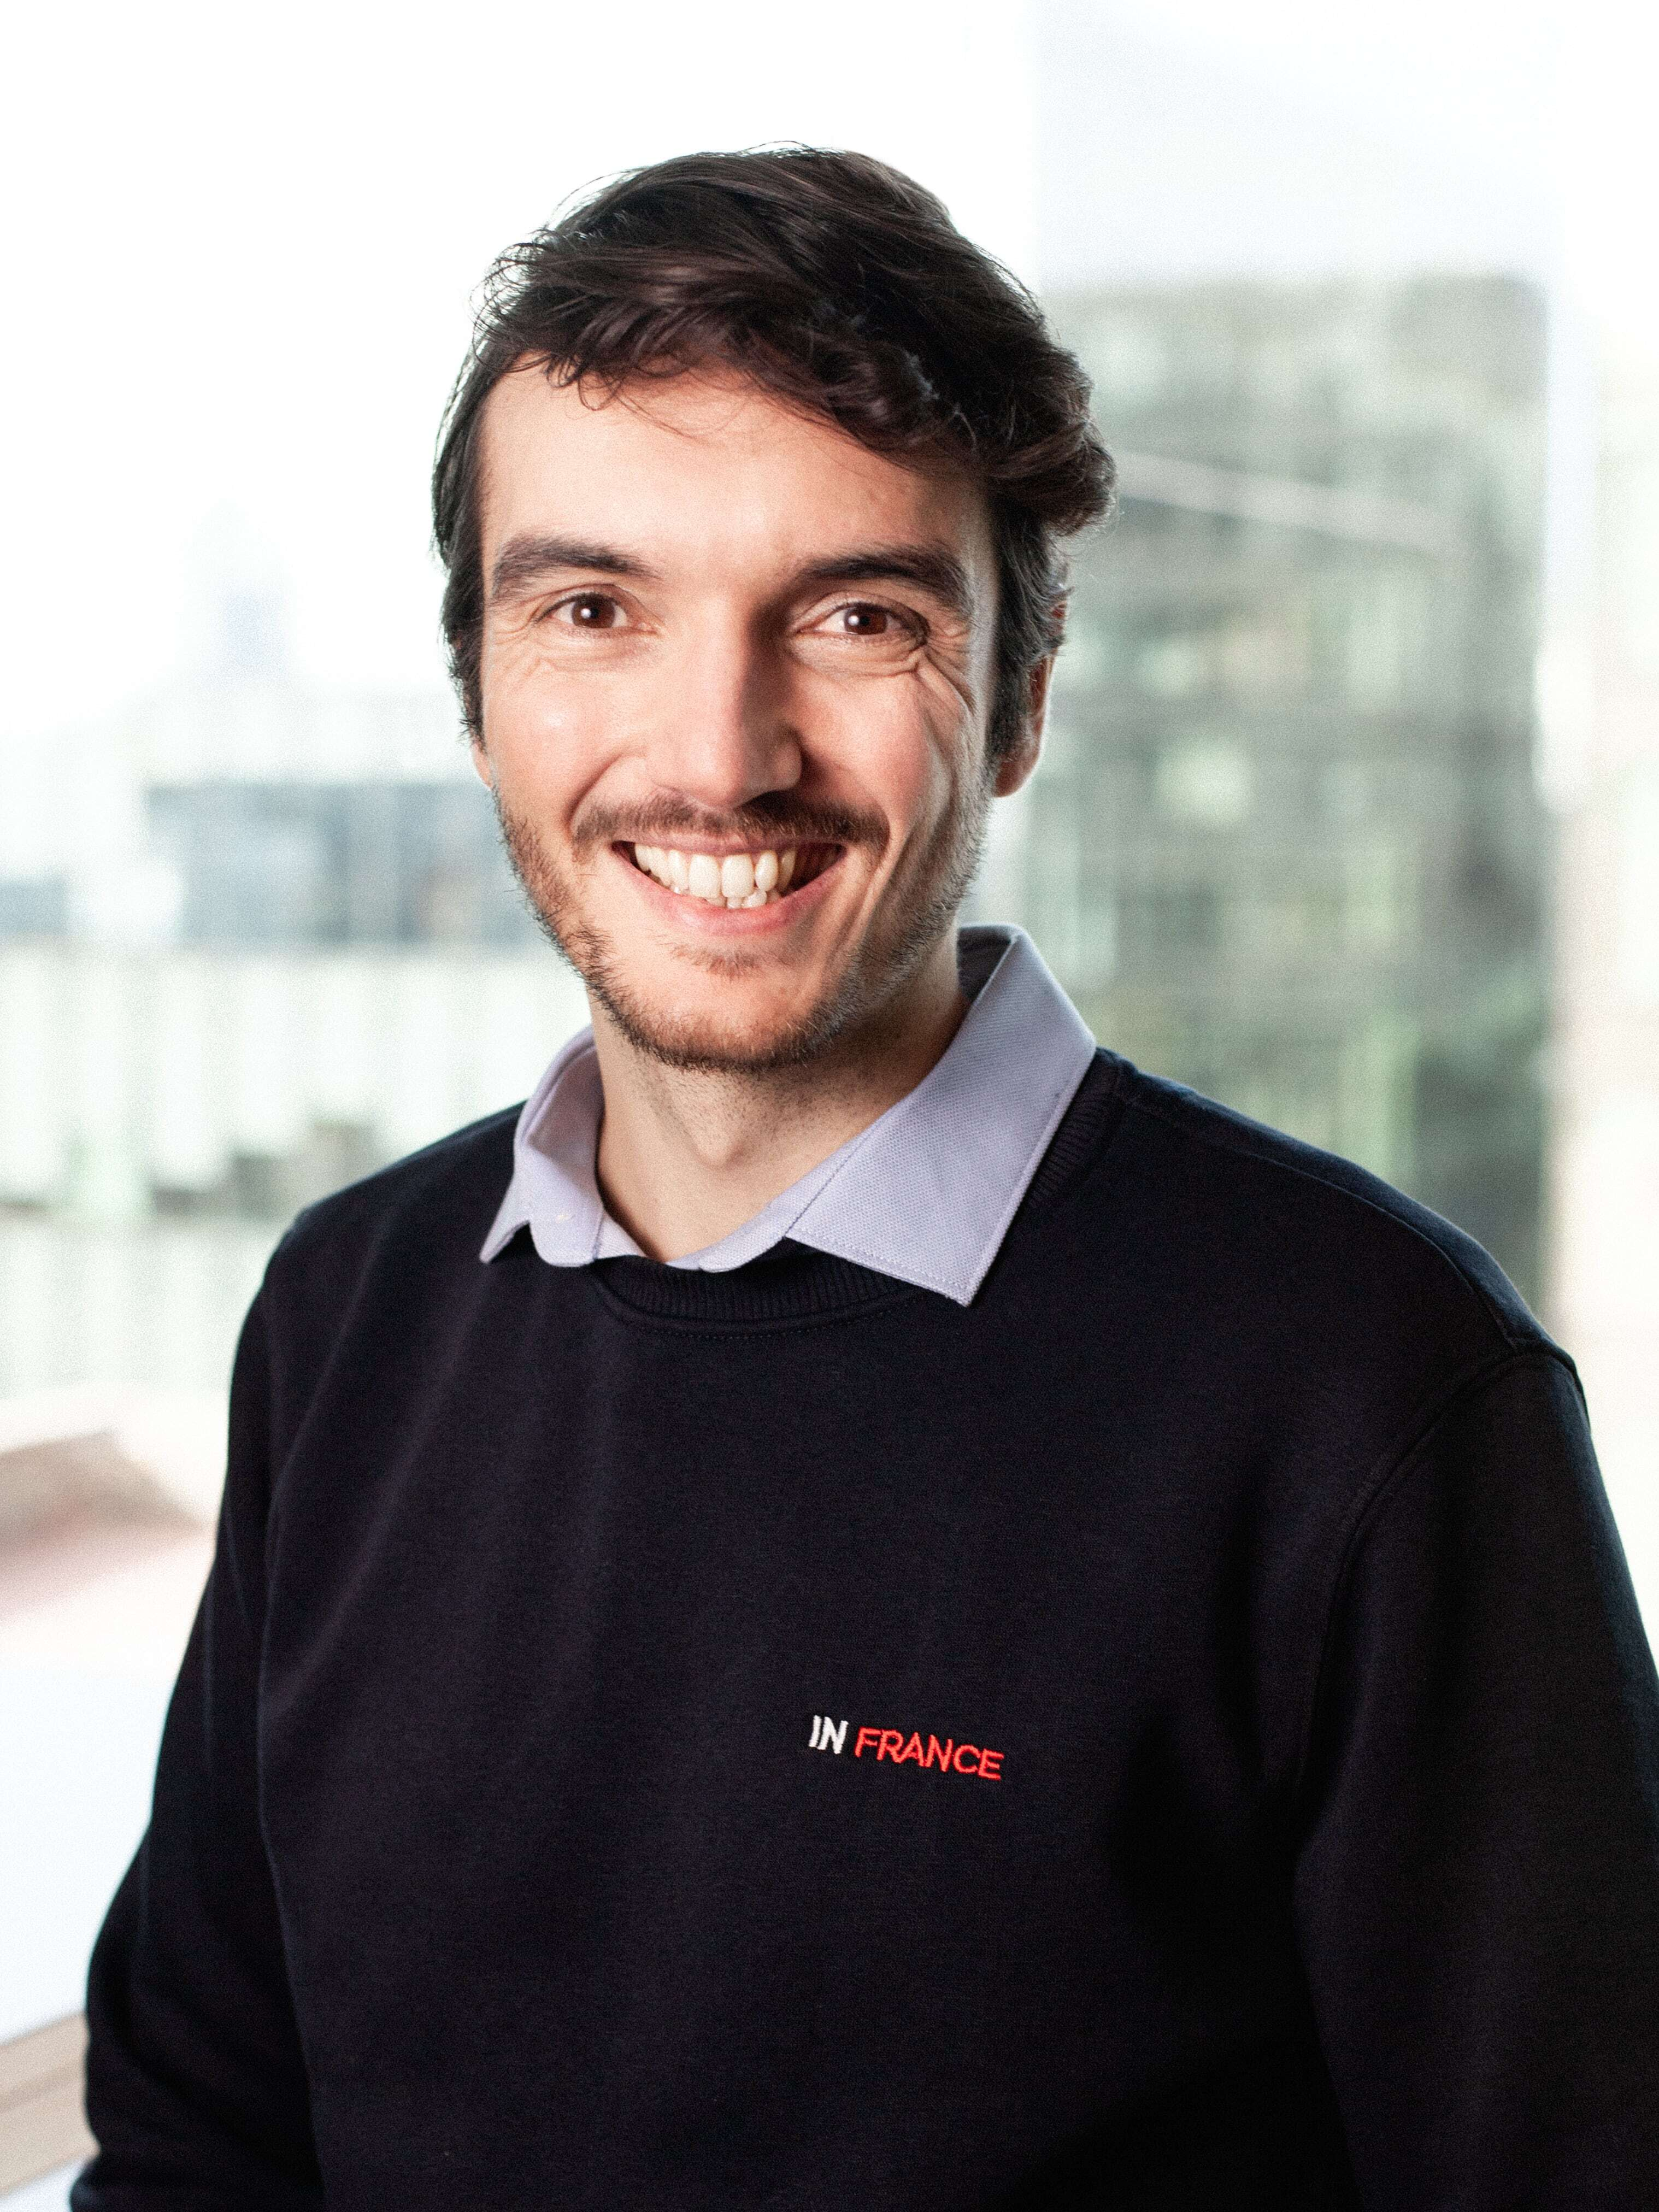
\includegraphics[width=5cm]{image/trombine-christophe}
        \end{columns}
    \end{frame}
    \begin{frame}{Pourquoi la Data Science en Python}{Les usages\footnote{\label{python-usage}Python usage in 2021 and 2022, \url{https://lp.jetbrains.com/python-developers-survey-2022/}}}
        \centering
        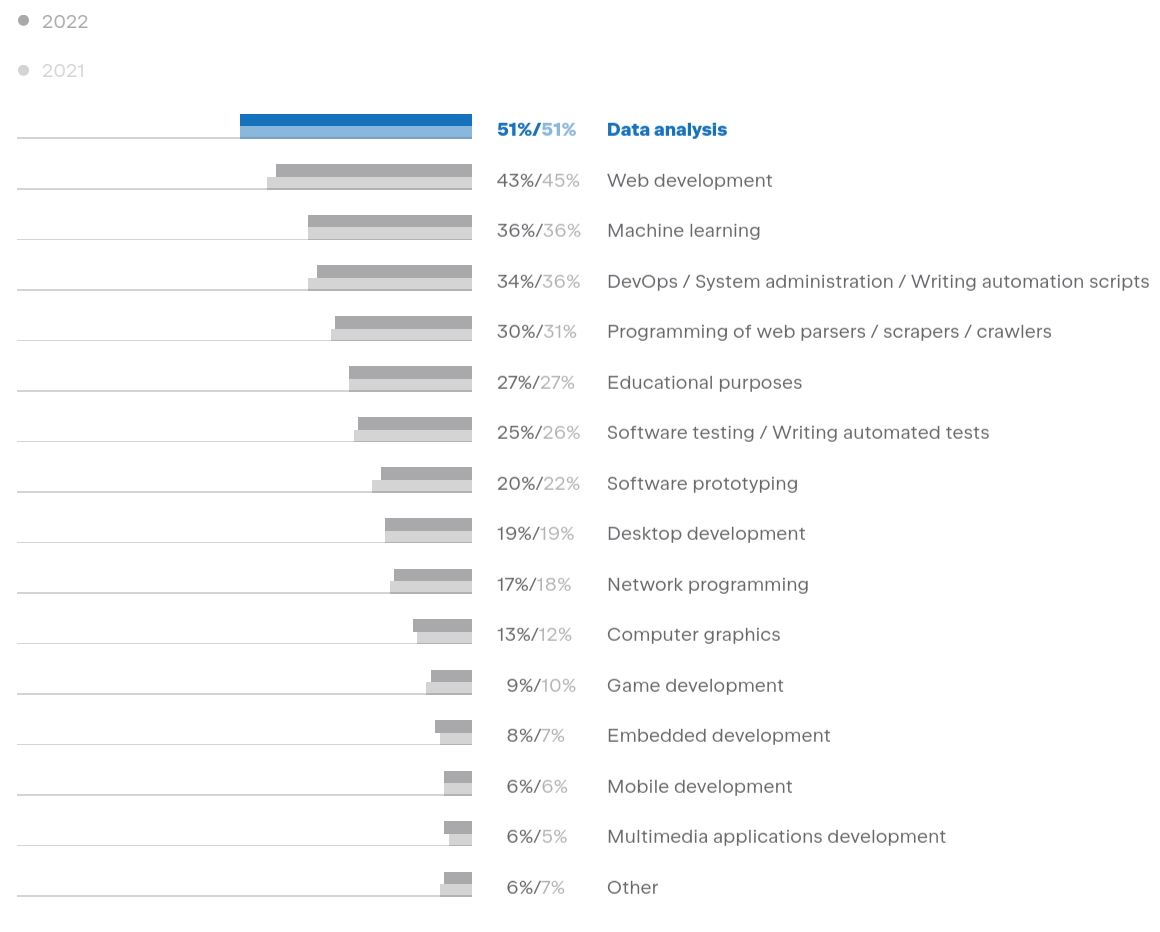
\includegraphics[width=8cm]{image/survey-usage}
    \end{frame}

    \begin{frame}{Quel Python~?}{L'interpréteur CPython domine\cref{python-usage}}
        \centering
        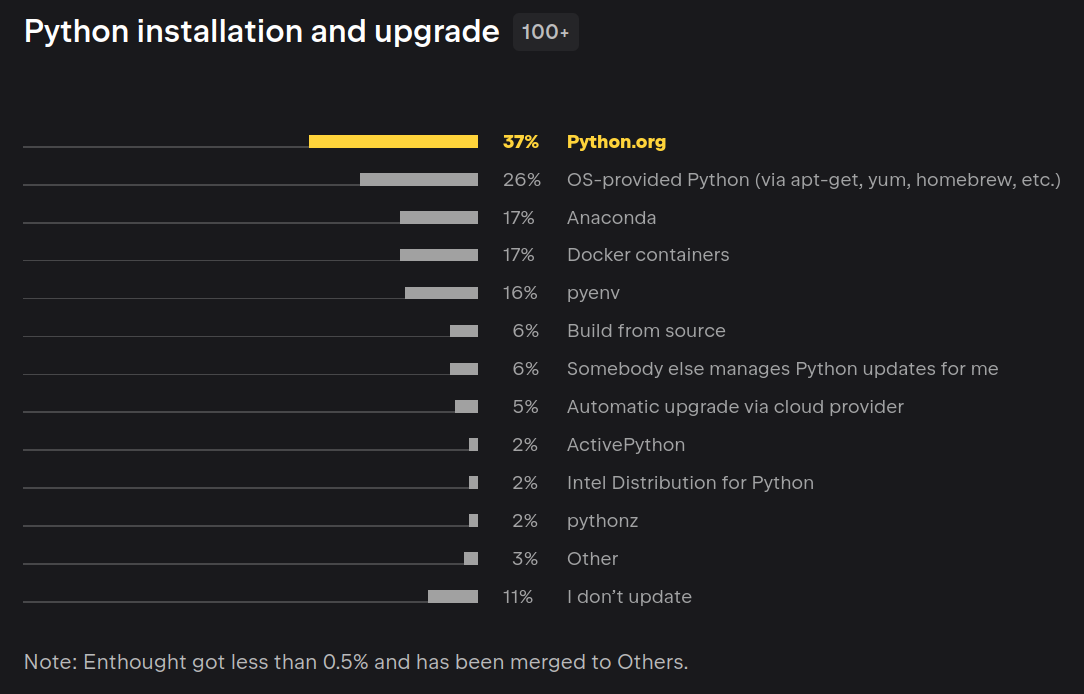
\includegraphics[width=10cm]{image/survey-install}
    \end{frame}

    \begin{frame}{Quel environnement de développement~?}{Les plus populaires\cref{python-usage}}
        \centering
        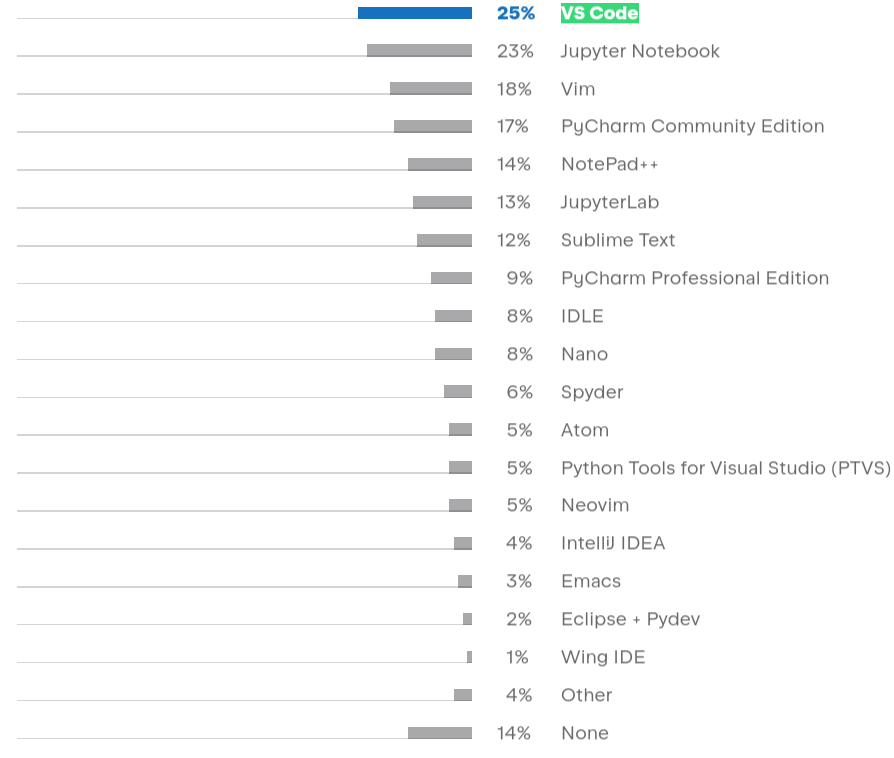
\includegraphics[width=9cm]{image/survey-ides}
    \end{frame}

    \begin{frame}{Quelques modules de la Standard Library}{Installer des packages distants}
        Où/Comment sont listées les dépendances Python~?
        \begin{center}
            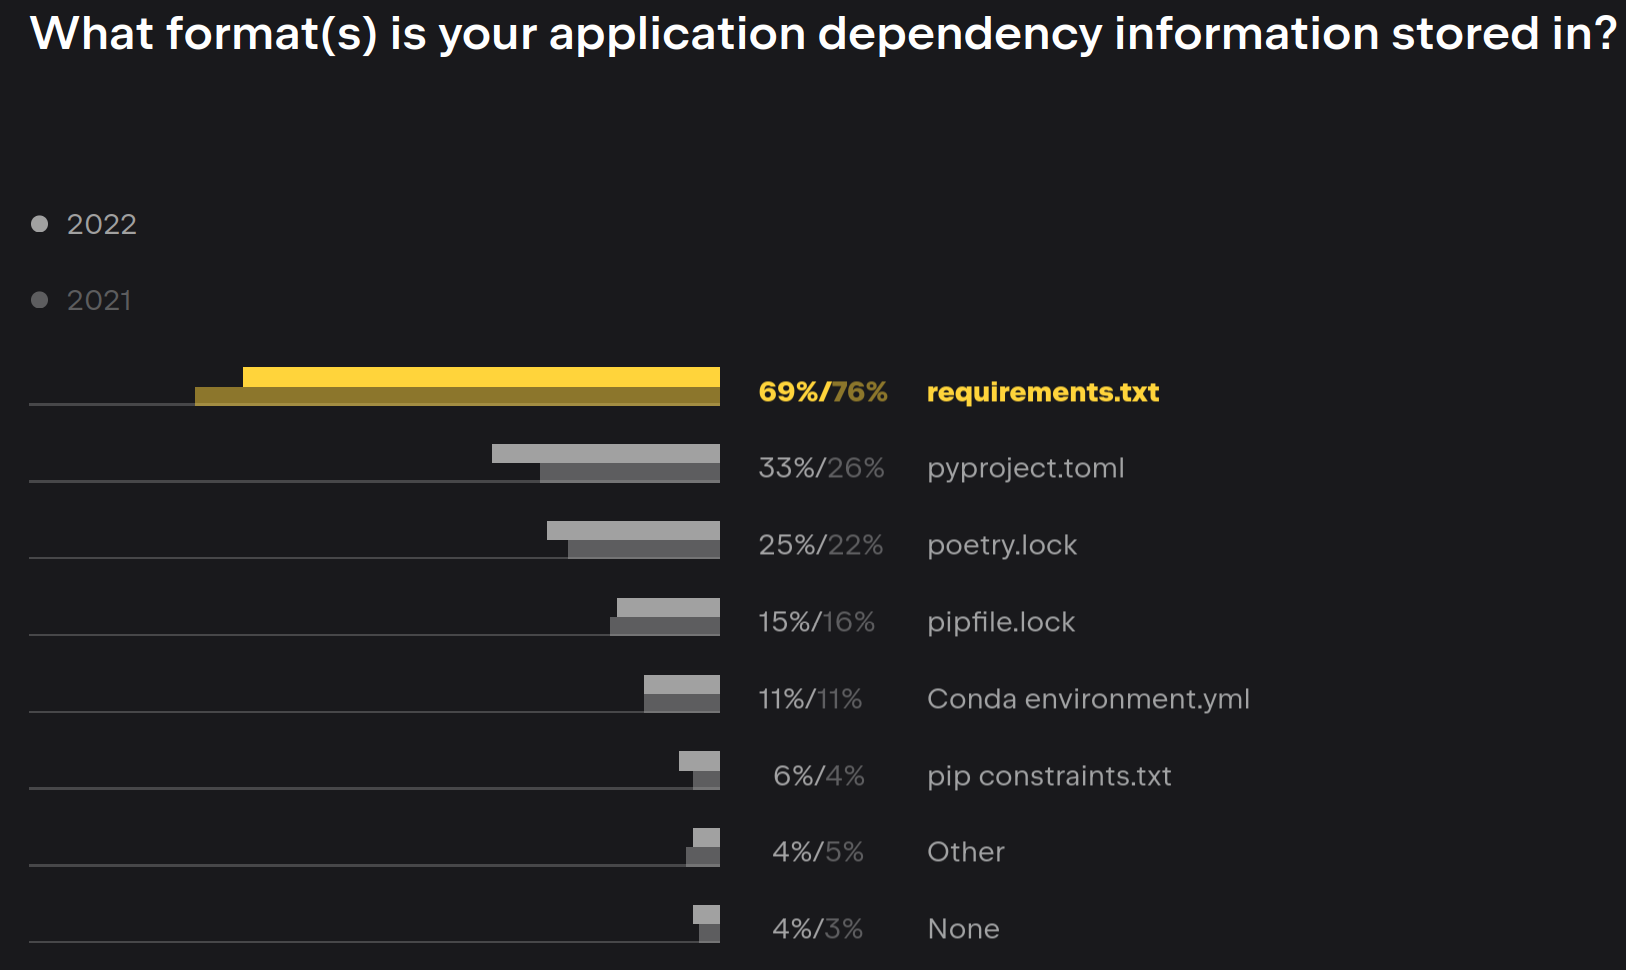
\includegraphics[width=10cm]{image/survey_dependency_listing}
        \end{center}
    \end{frame}


    \section{Jupyter Notebook}
    \begin{frame}{Jupyter Notebook}
        \begin{center}
            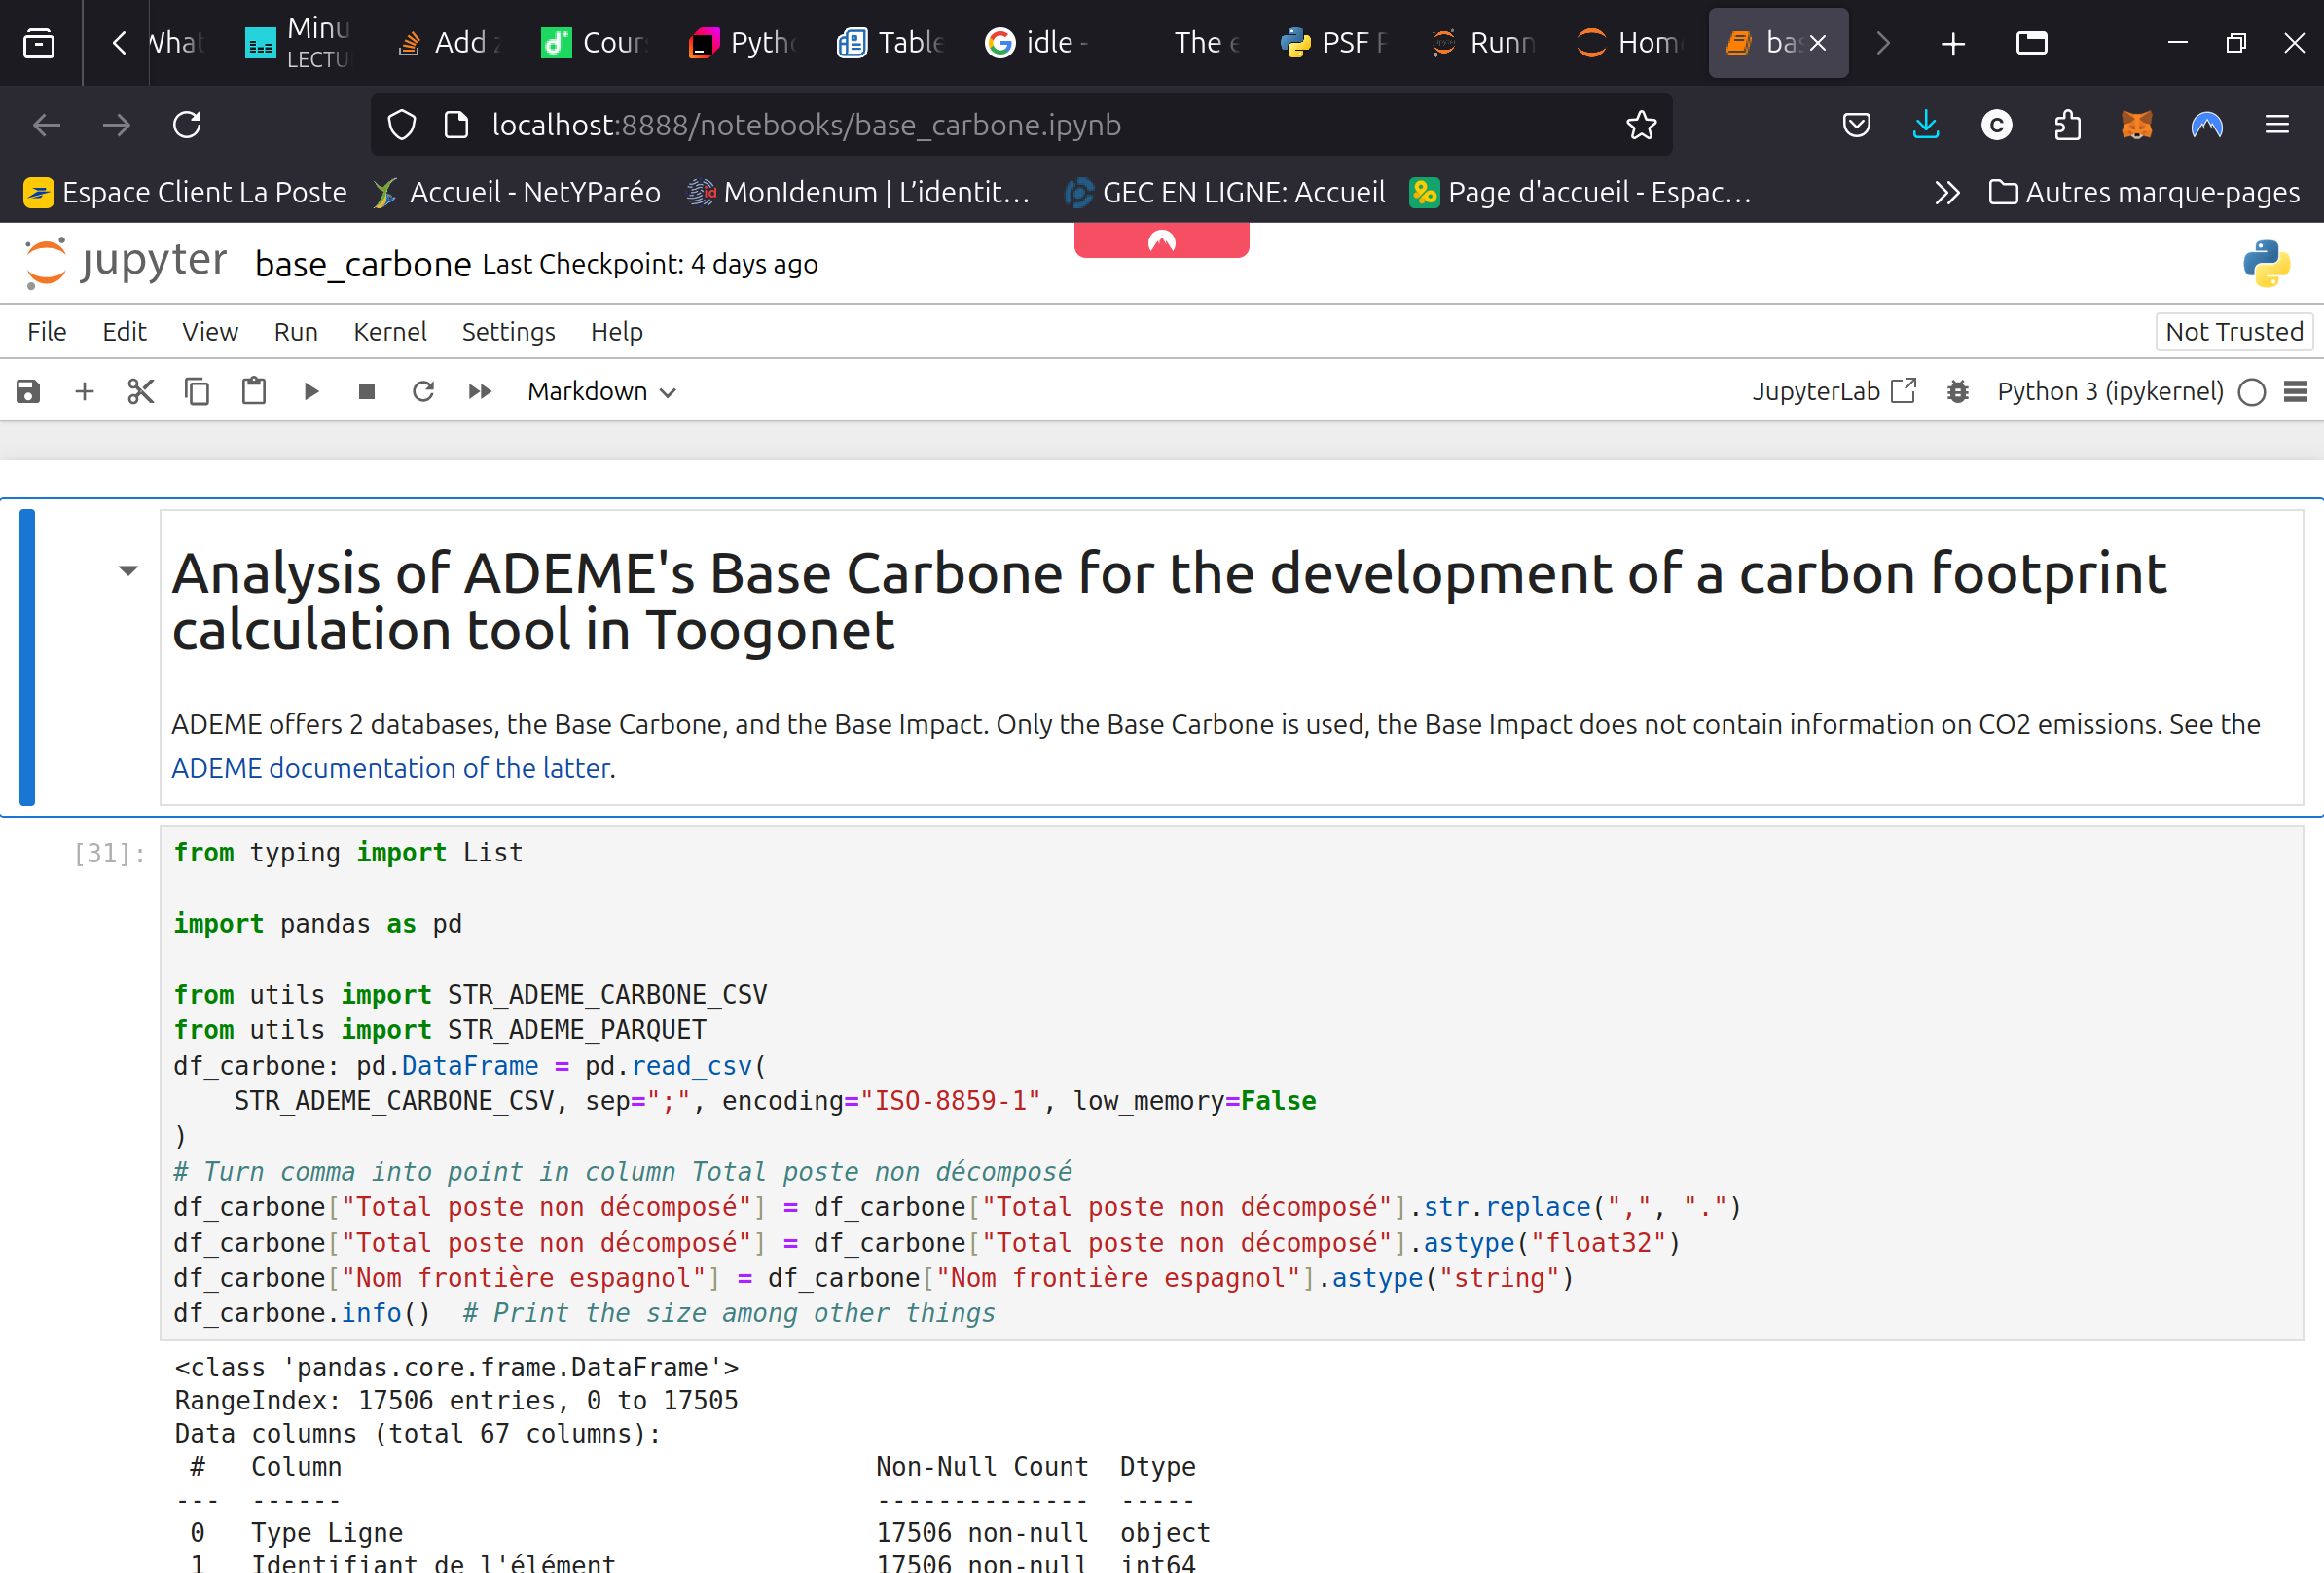
\includegraphics[width=12cm]{image/jupyter-notebook}
        \end{center}
    \end{frame}

    \begin{frame}{Jupyter Notebook}
        Le Jupyter Notebook est un environnement de développement interactif pour Python principalement, mais aussi d'autres langages.
        \bigbreak
        Il permet d'écrire des cellules de code, de le documenter dans des cellules en Markdown, de l'exécuter et de visualiser les résultats dans un même document.
        Par défaut, ce document est un fichier \lstinline{.ipynb} qui peut être ouvert et exécuté dans un navigateur web.
        Les données qu'il contient sont au format JSON, ses versions peuvent donc être suivies dans un VCS comme Git.
        Et même affiché sur les serveurs comme GitHub.
        \bigbreak
        Il est très utilisé en Data Science, \textit{etc} pour son interactivité et sa facilité d'utilisation.
        Par opposition à d'autre domaine de la programmation Python au web, testing qui utilisent un IDE
    \end{frame}

    \begin{frame}[fragile]{Jupyter Notebook}
        Techniquement, c'est un package Python qui execute du code Python dans un serveur web.
        On peut l'installer avec \lstinline{pip install jupyter} ou lister \lstinline{jupyter} dans le \lstinline{requirements.txt}.
        \bigbreak
        Il dépend en autre, de l'interpréteur IPython, un interpréteur Python 3 mais aussi un kernel Python qui permet d'exécuter du code Python dans un environnement Jupyter.
        Un kernel est un processus qui exécute le code et renvoie les résultats au client Jupyter.
        Il existe d'autres kernels qui peuvent s'intégrer au Notebook Jupyter comme Toree, pour utiliser d'autres langages de programmation comme Scala, R \ldots{}
        \bigbreak
        Toutes ces extension (Toree, IPyWidgets, \textit{etc}) sont également des packages Python qui peuvent être installés avec \lstinline{pip} ou listés dans le \lstinline{requirements.txt}.
    \end{frame}

    \subsection{Fonctionnement local, serveur, dans l'IDE}
    \begin{frame}{Jupyter Notebook}{Les environnements de développement}{Jupyter Notebook}{Notebook dans l'IDE, une aide précieuse}
        \begin{center}
            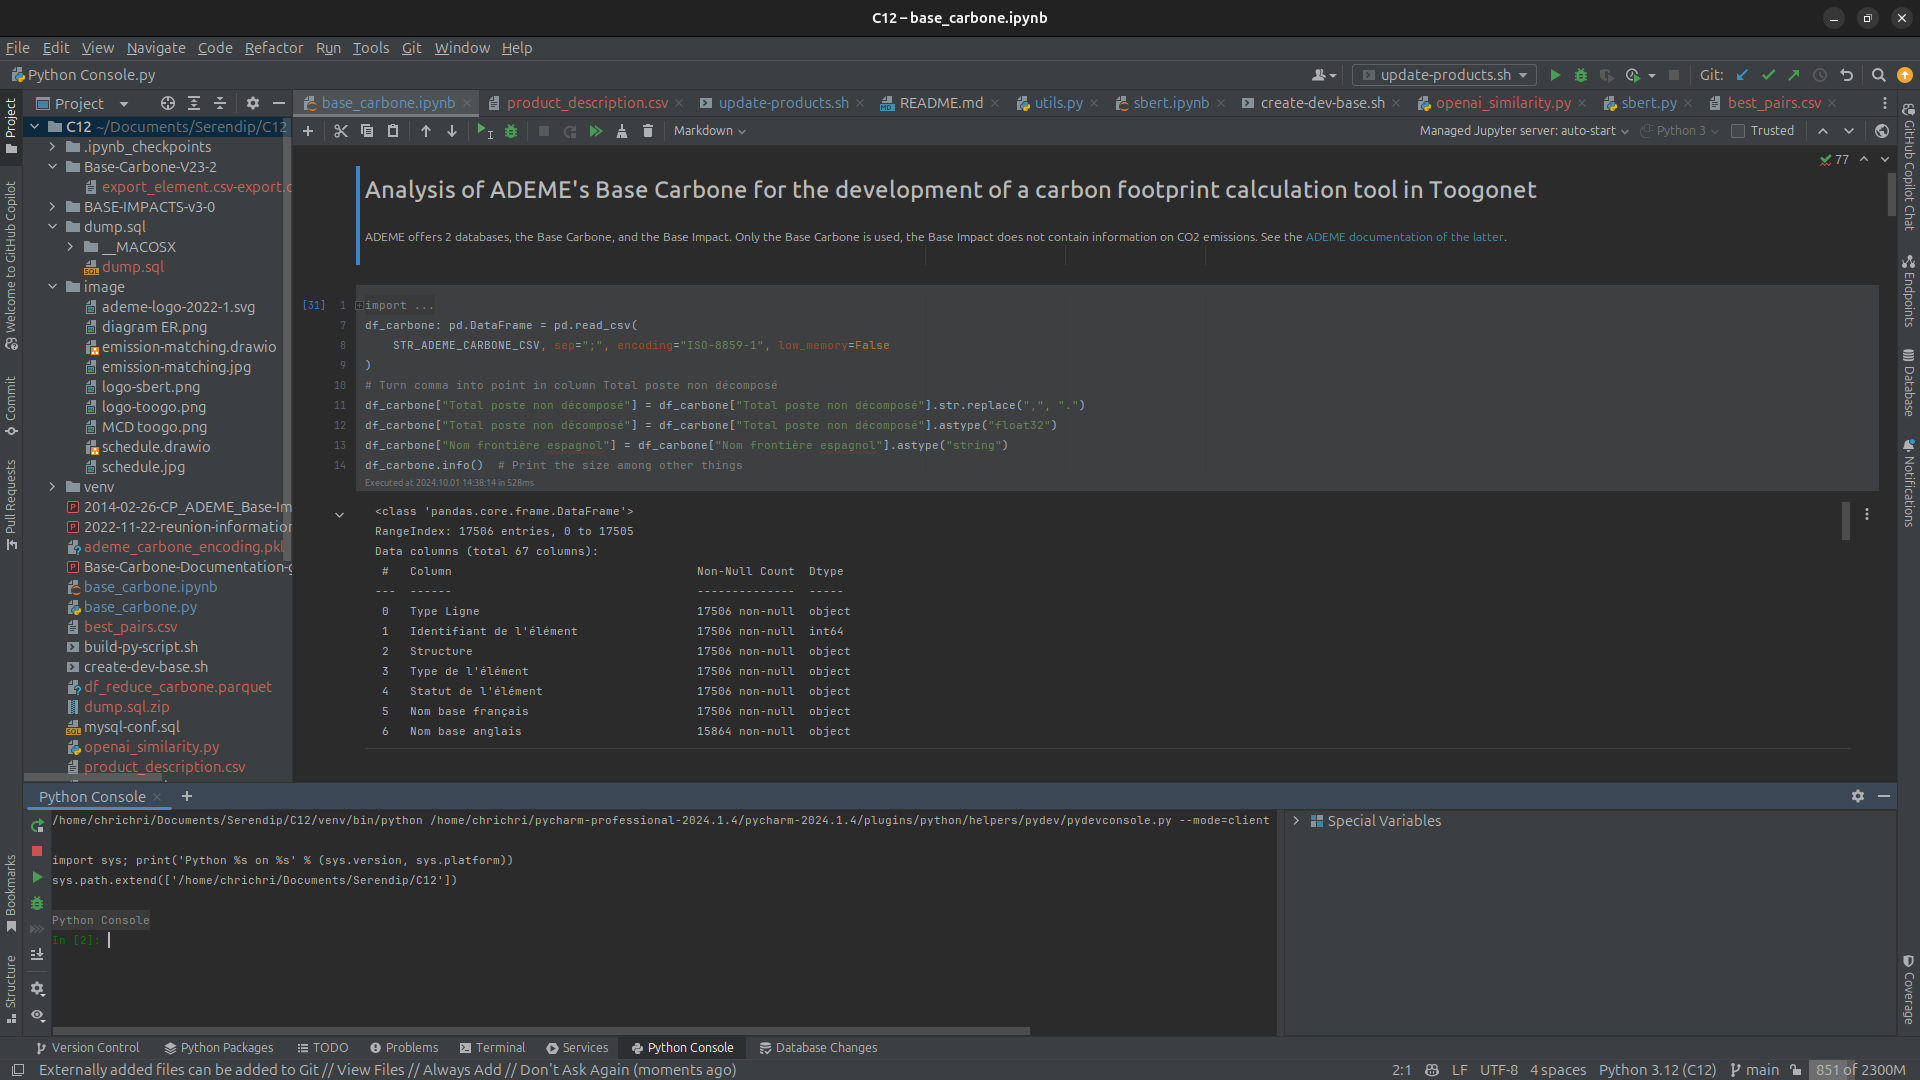
\includegraphics[width=9cm]{image/pycharm-notebook-repl}
        \end{center}
    \end{frame}

    \begin{frame}{Jupyter Notebook}{Notebook dans l'IDE, une aide précieuse}
        PyCharm est un freemium \url{https://www.jetbrains.com/pycharm/download/}, pour absolument tous usages~!
        \bigbreak
        IPython et Jupyter sont des packages qui s'installent à partir du gestionnaire de package de Python, \lstinline{pip}~:
        \begin{itemize}
            \item \lstinline{pip install ipython}
            \item \lstinline{pip install jupyter}, mais cette commande est à privilégier dans un virtual environnement.
            Un virtual environnement est un environnement Python isolé, qui permet de ne pas polluer l'environnement global de Python.
        \end{itemize}
    \end{frame}


    \begin{frame}{Jupyter Notebook}{Notebook dans l'IDE, une aide précieuse}
        \begin{columns}
            \column{0.5\textwidth}
            \begin{center}
                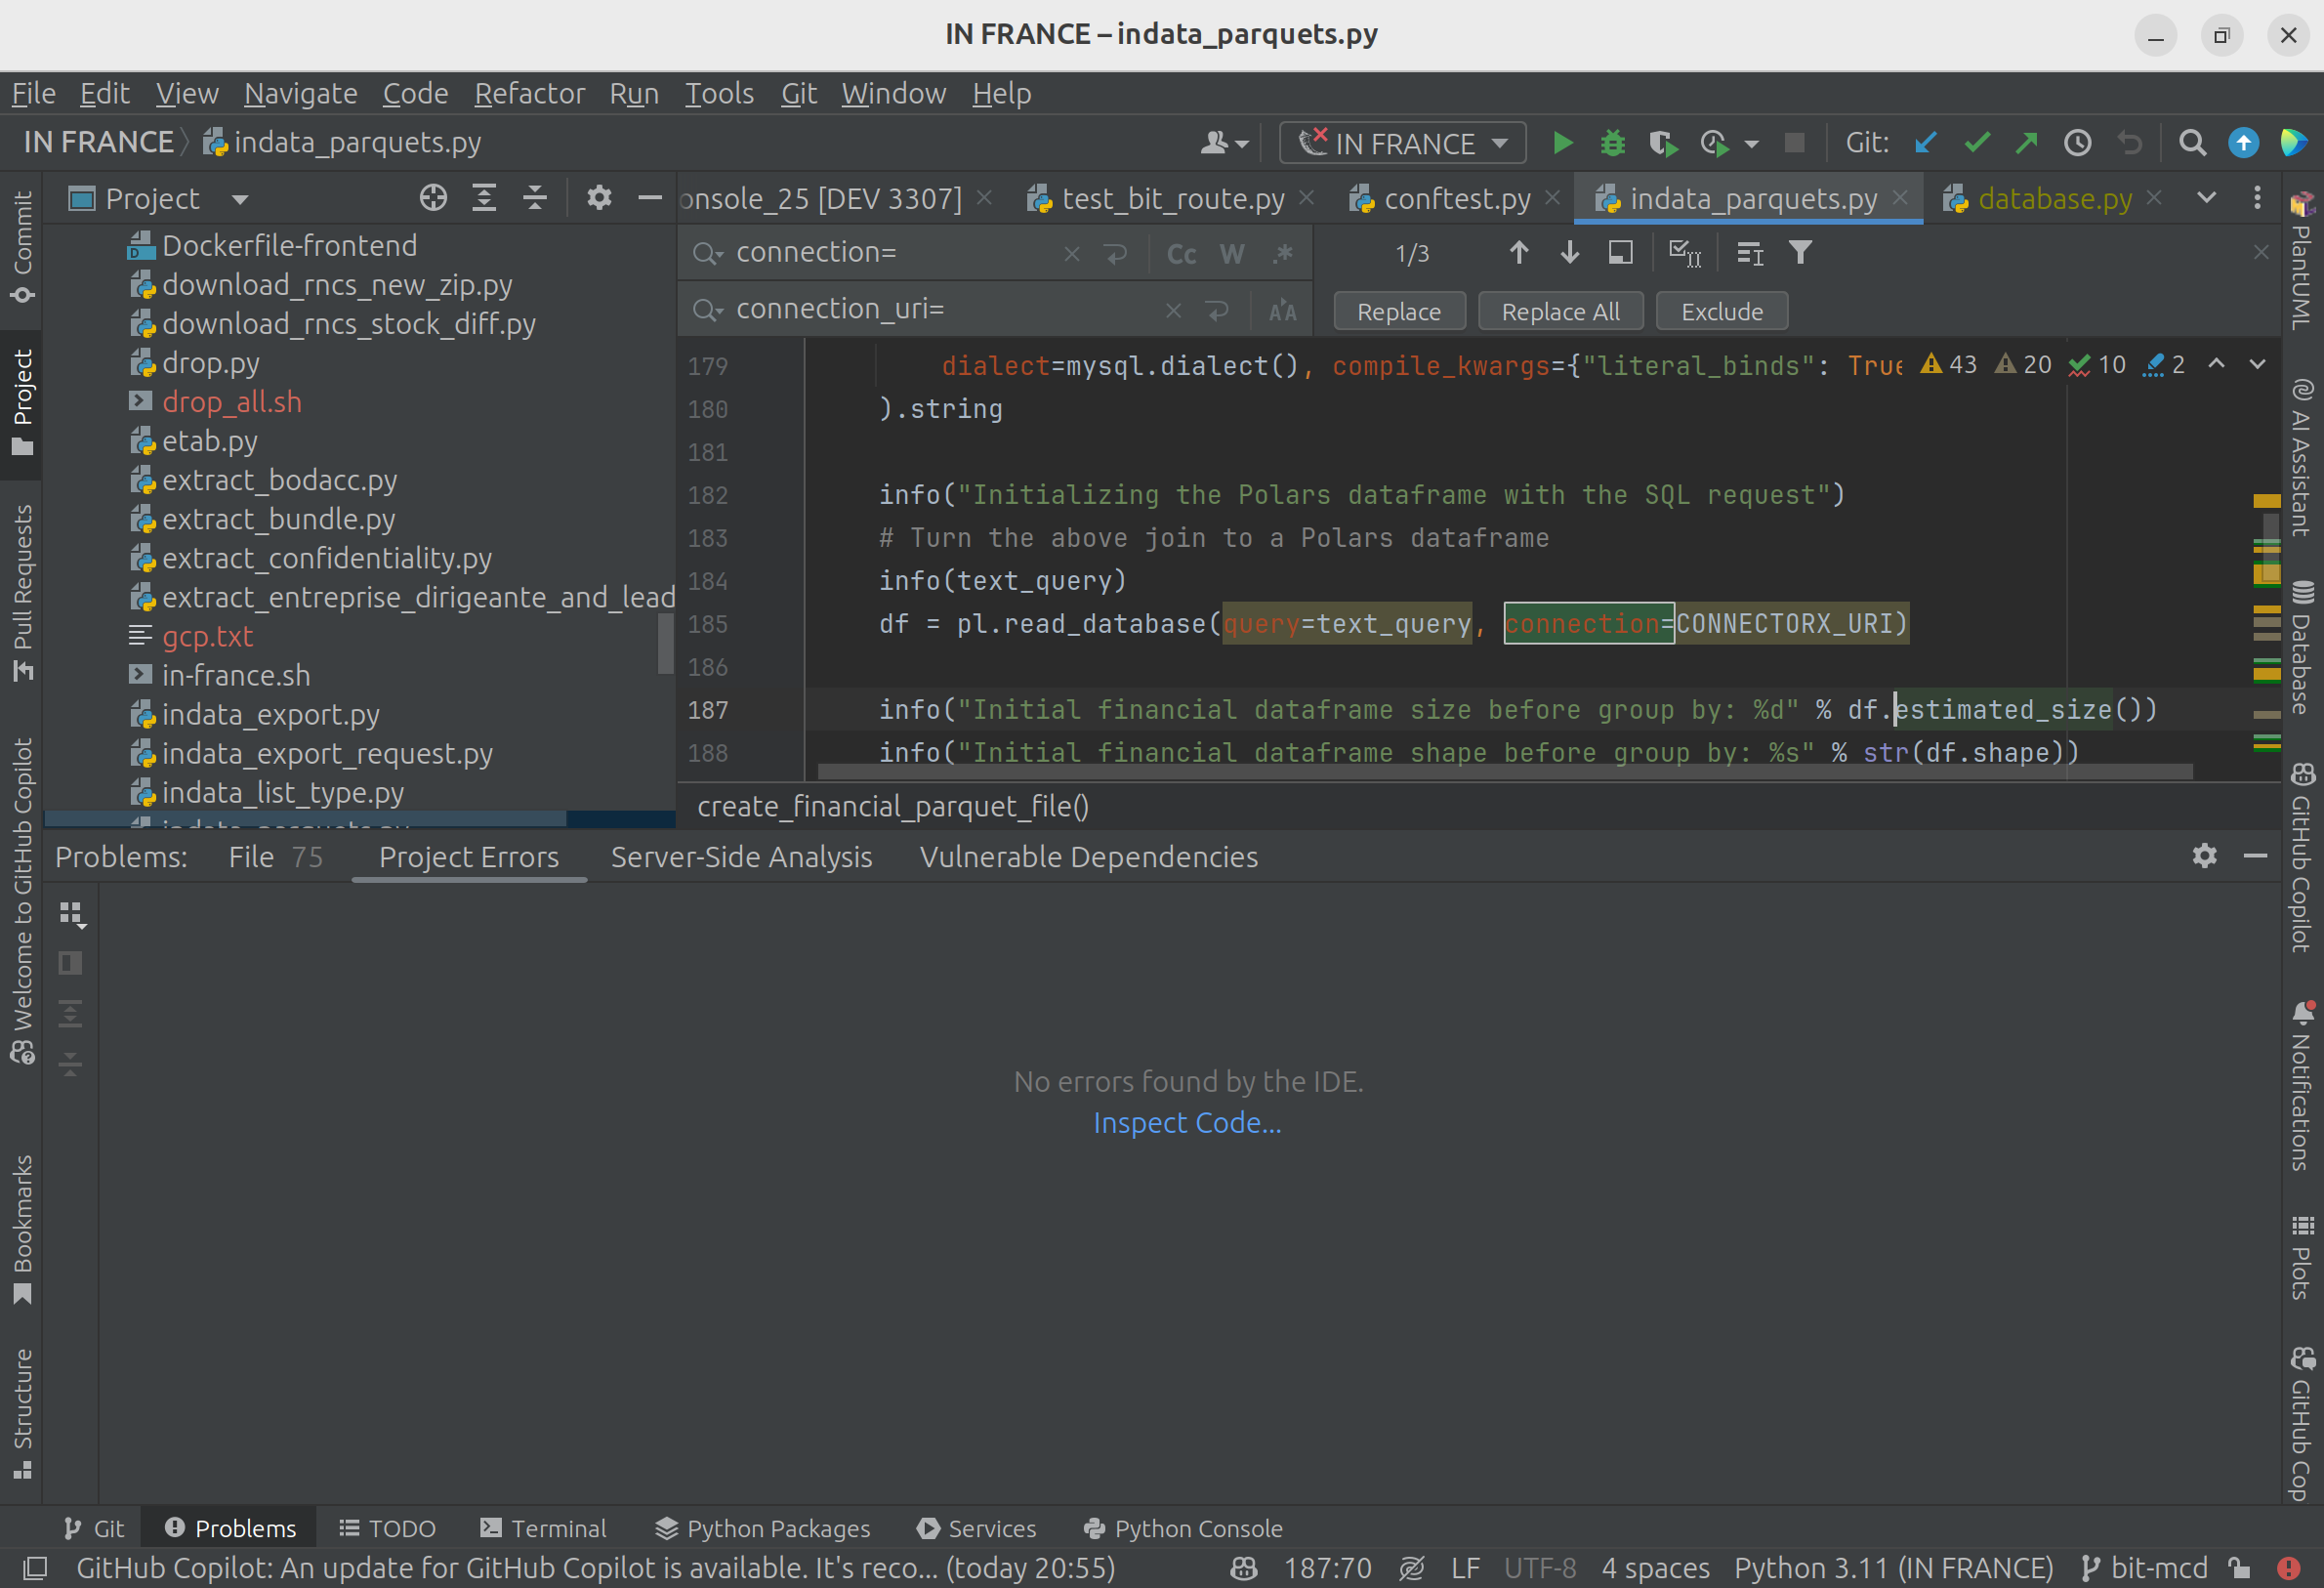
\includegraphics[width=5cm]{image/Pycharm-before-analysis}
            \end{center}
            \column{0.5\textwidth}
            \begin{center}
                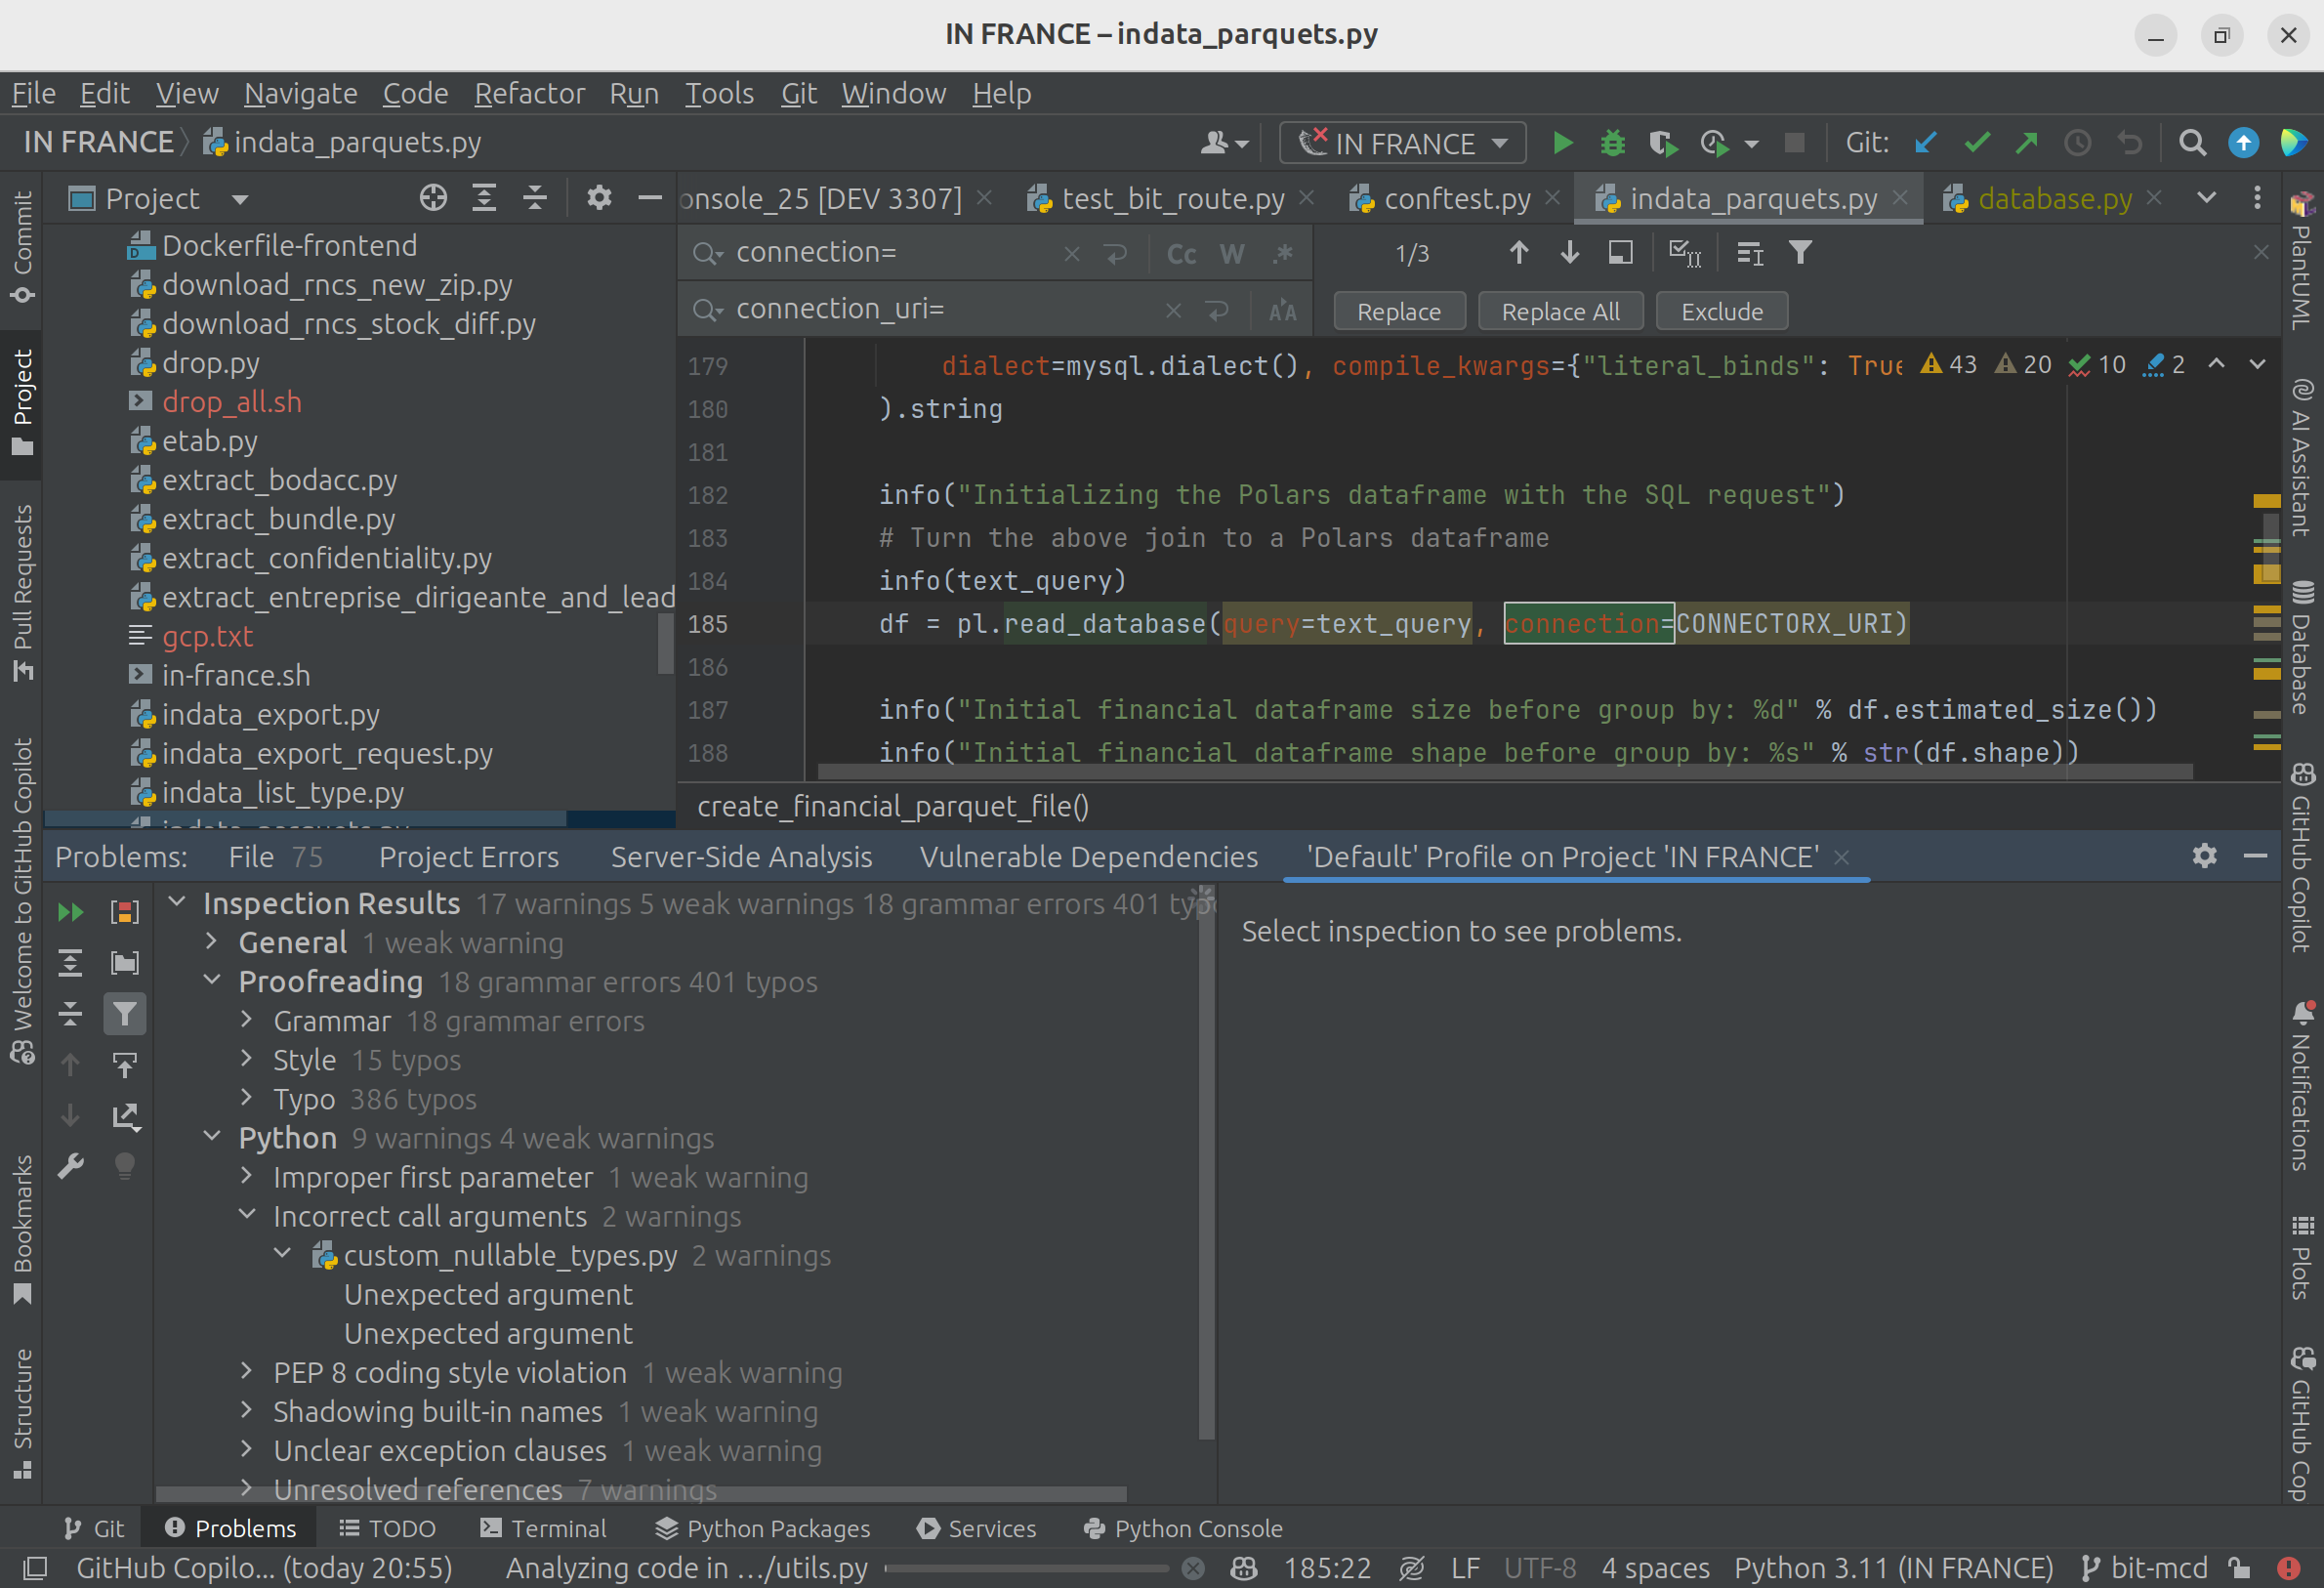
\includegraphics[width=5cm]{image/Pycharm-after-analysis}
            \end{center}
        \end{columns}
        \begin{dangercolorbox}
            Pycharm ou VS Code ont un débuggeur, le Notebook n'en n'a pas~!
        \end{dangercolorbox}
    \end{frame}

    \subsection{Interface et commandes}
    \begin{frame}{Jupyter Notebook}{Interface et commandes\footnote{Jupyter Notebook tips and shortcuts, \url{https://digitalhumanities.hkust.edu.hk/tutorials/jupyter-notebook-tips-and-shortcuts/}}}
        \footnotesize
        Le server Jupyter se lance avec la commande \lstinline{python -m jupyter notebook} dans un terminal, sinon dans l'IDE.
        \begin{itemize}
            \footnotesize
            \item \textbf{Mode commande (Bleu)}~:
            \begin{itemize}
                \footnotesize
                \item \texttt{A}~: Insérer une cellule \textbf{au-dessus}
                \item \texttt{B}~: Insérer une cellule \textbf{en dessous}
                \item \texttt{D, D}~: Supprimer la cellule
                \item \texttt{Z}~: Restaurer la dernière cellule supprimée
                \item \texttt{Y}~: Passer la cellule en mode \textbf{code}
                \item \texttt{M}~: Passer la cellule en mode \textbf{markdown}
                \item \texttt{Enter}~: Passer en mode édition
            \end{itemize}

            \item \textbf{Mode édition (Vert)}~:
            \begin{itemize}
                \footnotesize
                \item \texttt{Alt + Enter}~: Exécuter et insérer une nouvelle cellule
                \item \texttt{Esc}~: Sortir du mode édition (revenir au mode commande)
            \end{itemize}
            \item \textbf{Dans tous les modes}
            \begin{itemize}
                \footnotesize
                \item \lstinline{!} en début d'une ligne d'une cellule permet d'ajouter un commande Shell, sorting du Shell Python.
                \item \texttt{Ctrl + Enter}~: Exécuter la cellule
                \item \texttt{Shift + Enter}~: Exécuter et passer à la suivante
            \end{itemize}
        \end{itemize}
    \end{frame}

    \subsection{Comment coder dans un Notebook~?}\label{jupyter-coding-style}
    \begin{frame}[fragile]{Jupyter Notebook}{Comment coder dans un Notebook~?}
        \small
        \begin{dangercolorbox}
            Faire usage des bonnes pratiques de développement logiciel et Python (PEP).
            \textbf{Être dans la data science n'excuse rien~!}

            Si les données, les data visualizations, sont validés par l'équipe, il est important de pouvoir les extraire tel quelles du Notebook pour ne pas recoder et introduire un bug.
            Dans le CI/CD en tant qu'artefact par exemple.
        \end{dangercolorbox}
        \bigbreak
        Si on définit des structures comme des classes ou des fonctions, sachant que le code du Notebook peut être extrait en une ligne de commande.
        Il est possible de porter ses structures dans un dashboard web, un script de manipulation de données, \textit{etc}.
        \begin{lstlisting}[language=bash]
jupyter nbconvert --to script mon_notebook.ipynb
        \end{lstlisting}
        \begin{center}
            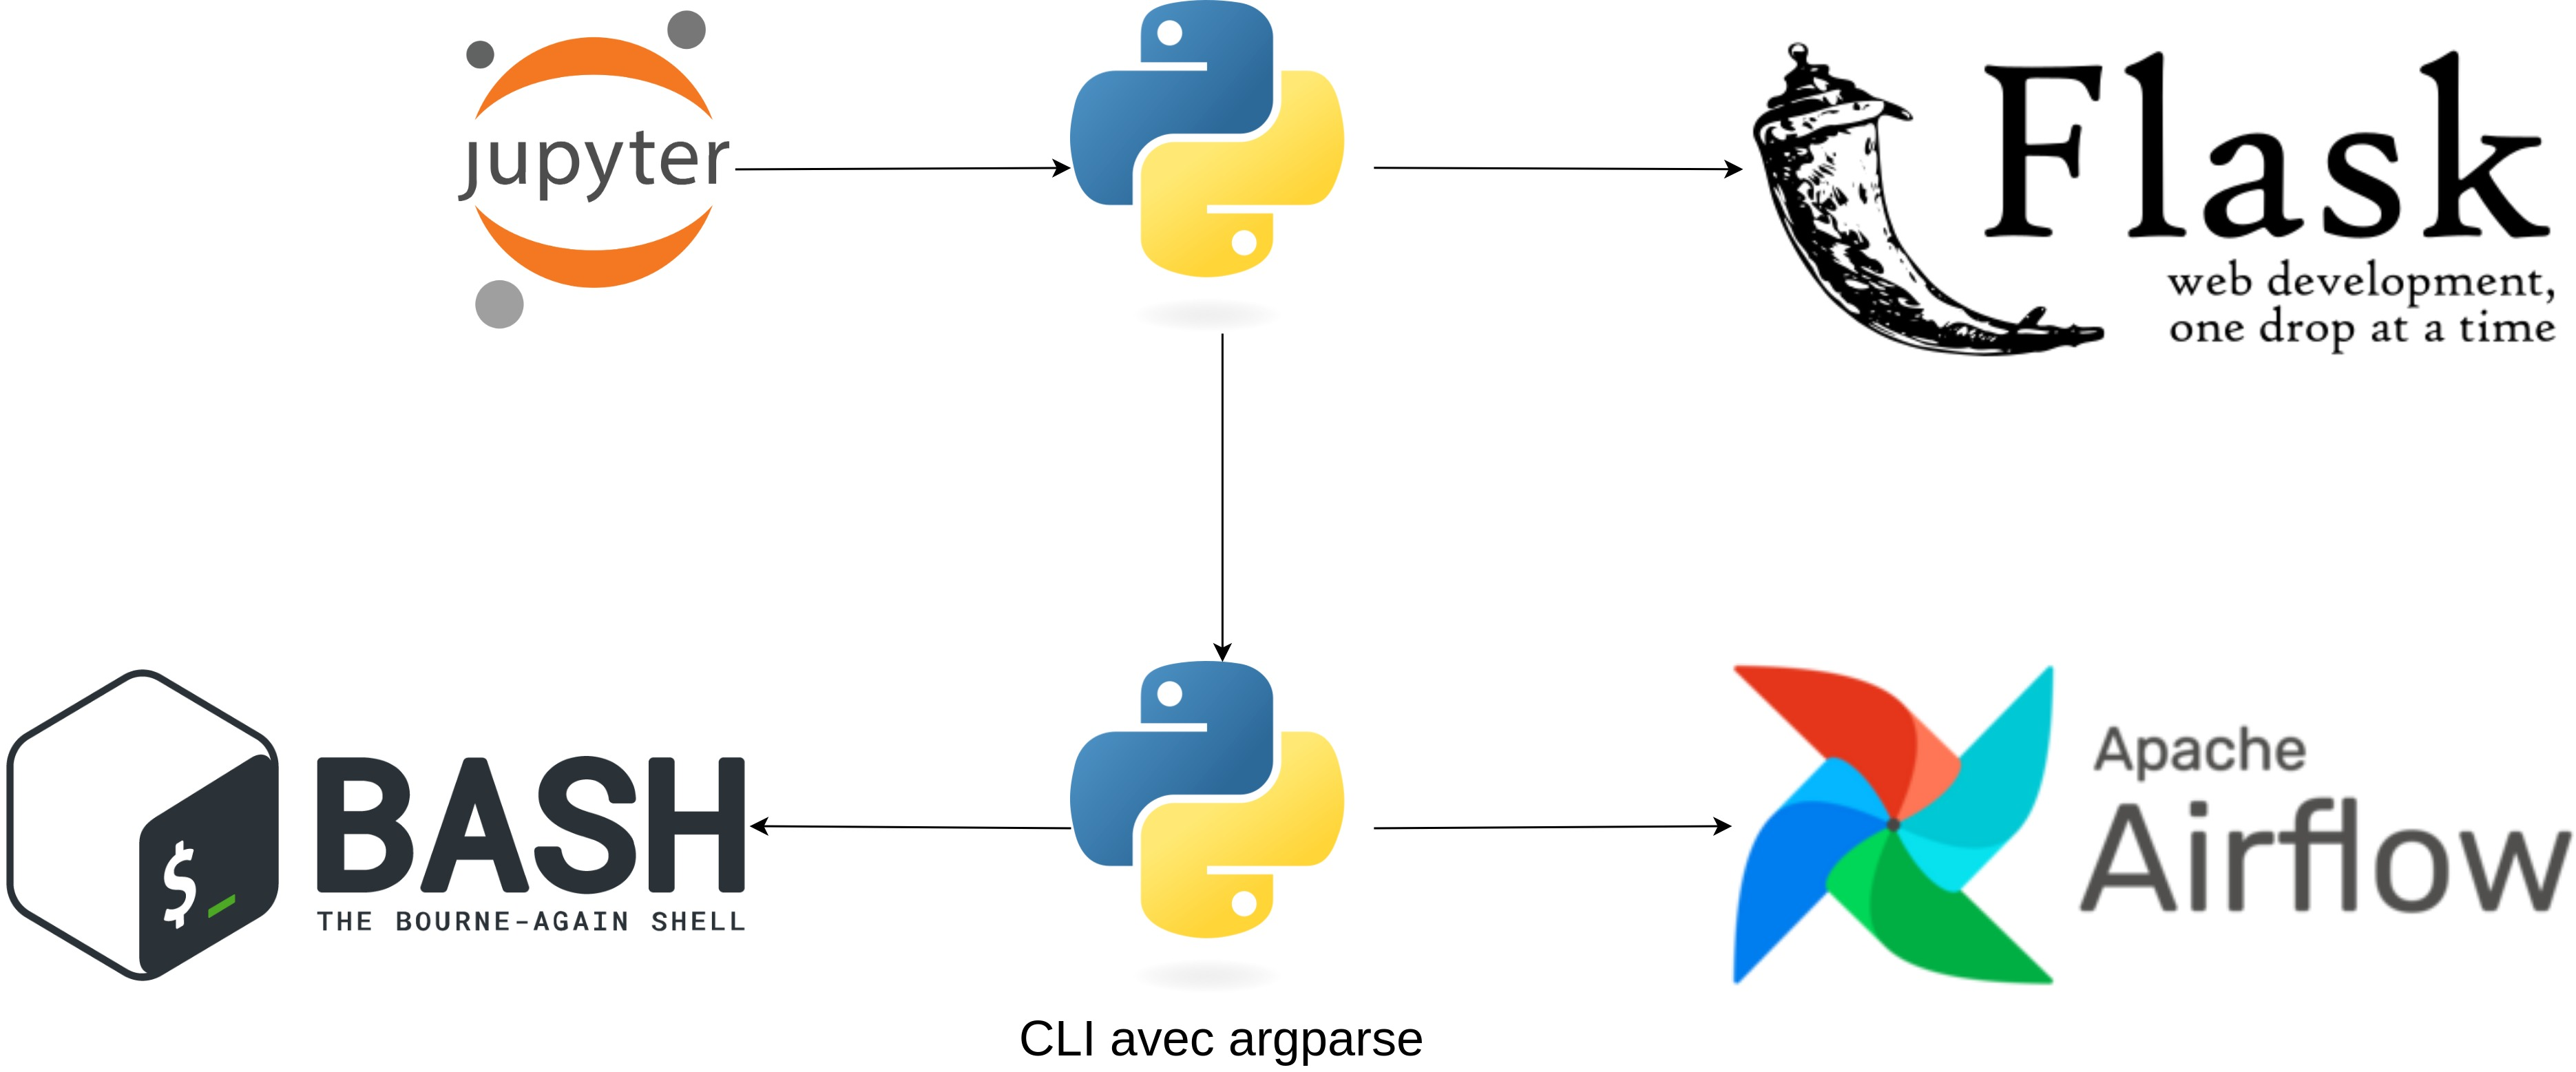
\includegraphics[width=6cm]{image/from-notebook-to-production}
        \end{center}
    \end{frame}

    \subsection{Notebook Jupyter en ligne avec Voilà}
    \begin{frame}[fragile]{Jupyter Notebook}{Voilà}{Interface Web pour Notebooks Jupyter\footnote{voilà, \url{https://voila.readthedocs.io/}}}
        \begin{itemize}
            \item Outil pour transformer un notebook Jupyter en une application web interactive.
            Passer d'un prototype à un vrai dashboard sur le réseau de l'entreprise.
            \item Cache le code source pour ne montrer que les widgets et résultats.
            \item Utiliser des thèmes pour personnaliser l'apparence.
            \item Installation~:
            \begin{lstlisting}[language=bash,basicstyle=\tiny\ttfamily]
pip install voila
            \end{lstlisting}
            \item Utilisation~:
            \begin{lstlisting}[language=bash,basicstyle=\tiny\ttfamily]
voila mon_notebook.ipynb
# Supprime la sortie d'une cellule taggé avec hide
voila --TagRemovePreprocessor.remove_all_outputs_tags='{"hide"}' mon_notebook.ipynb
# Supprime une cellule taggé avec hide
voila --TagRemovePreprocessor.remove_cell_tags='{"hide"}' mon_notebook.ipynb
            \end{lstlisting}
        \end{itemize}
    \end{frame}

    \subsection{Exercice}\label{jupyter-exercice}
    \begin{frame}{Jupyter Notebook}{Exercice \execcounterdispinc{}}
        \begin{itemize}
            \item Télécharger le code du cours sur l'URL \url{https://github.com/DigicompClassesByPapIT/PYDATA}.
            \item Créer un virtual environnement Python dans ce dossier.
            \item Vérifier que la librairie \lstinline{jupyter} est listée comme dépendance.
            \item Installer les dépendances.
            \item Créer un Notebook.
            \item Exécuter les cellules du Notebook.
            \item Utiliser les commandes Voilà pour le transformer en application web.
        \end{itemize}
    \end{frame}


    \section{Programmation fonctionnelle}

    \subsection{Expressions lambda}
    \begin{frame}[fragile]{Expressions lambda}{Map, filter et reduce}
        Il existe de nombreux langages fonctionnels~: Haskell, Lisp, Erlang, Scala, F\#.
        \bigbreak
        D'autres langages supportent la programmation fonctionnelle comme Python, JS, Java en autres et ont des outils/librairies dédiées à la programmation fonctionnelle.
        \bigbreak
        La programmation fonctionnelle est un paradigme de programmation qui utilise des fonctions comme unités de base.
        Ces fonctions sont séparées en deux types~:
        \begin{itemize}
            \item Les fonctions pures, qui ne modifient pas l'état du programme et ne dépendent pas de l'état du programme.
            \item Les fonctions impures ou avec effet de bord, qui modifient l'état du programme ou de la machine (affichage) ou dépendent de l'état du programme, d'une condition extérieure\ldots{}
        \end{itemize}
        Souvent nommées fonctions lambda venant du \textit{lambda calculus}.
        Ces expressions sont associées à map, reduce, filter, etc.
    \end{frame}

    \begin{frame}{Expressions lambda}{Pourquoi des fonctions et non des objets}
        Scala prétend que la programmation fonctionnelle permet une mise à l'échelle plus facile des gros projets.
        D'où sont nom, Scala pour \textit{SCAlable LAnguage}.

        Mais Pourquoi~?
        \bigbreak
        \begin{itemize}
            \item Les attributs des objets peuvent être modifiés à divers endroits du code, ce qui rend le code difficile à comprendre et à maintenir.
            Ce système n'est pas \textit{stateless}.
            \item Les fonctions pures n'ont pas d'état, elles ne modifient pas l'état du programme.
            Elles sont donc \textit{stateless} et serait plus faciles à comprendre et à
        \end{itemize}
        \begin{dangercolorbox}
            PEP décourage l'usage des fonctions anonymes\footnotemark~!
        \end{dangercolorbox}
        \footnotetext{https://peps.python.org/pep-0008/\#programming-recommendations}
    \end{frame}

    \begin{frame}[fragile]{Expressions lambda}{Map, Reduce et Filter}
        \begin{footnotesize}
            3 modules dédiés à la programmation fonctionnelle dans la \textquote{standard library} Python\footnote{Functional Programming Modules, \url{https://docs.python.org/3/library/functional.html}}~:
            \begin{itemize}
                \item \lstinline{functools}, \textquote{Higher-order functions and operations on callable objects}.
                \item \lstinline{itertools}, \textquote{Functions creating iterators for efficient looping}.
                \item \lstinline{operator}, \textquote{Standard operators as functions}.
            \end{itemize}
            \begin{lstlisting}[language=bash]
>>> is_even = lambda x: x % 2 == 0 # No return needed?
>>> list(map(is_even, [1, 2, 3, 4]))
[False, True, False, True]
>>> list(filter(is_even, [1, 2, 3, 4])) # Kept only if True
[2, 4]
>>> from functools import reduce
>>> from operator import mul
>>> reduce(mul, [1, 2, 3, 4]) # Function applied to all elements, 1 * 2 * 3 * 4
24
            \end{lstlisting}
        \end{footnotesize}
    \end{frame}

    \subsection{List comprehension}

    \begin{frame}[fragile]{List comprehension}
        Les \textit{list comprehension} sont une manière concise de créer des listes en Python en appliquant une transformation et/ou un filtre à une séquence existante.
        Elles sont souvent utilisées pour remplacer les boucles \lstinline{for} et les fonctions \lstinline{map} et \lstinline{filter}.
        \bigbreak
        Exemple d'une fonction qui nettoie du text en ne gardant que les mots de plus de 3 caractères et élimine la case~:
        \begin{lstlisting}[language=bash,basicstyle=\tiny\ttfamily]
# Avec boucle for classique
words = ['data', 'AI', 'python', 'ML', 'visualization']
capitalized_long_words = []
for word in words:
    if len(word) > 3:
        capitalized_long_words.append(word.upper())

# Avec map et filter
capitalized_long_words = list(map(str.upper, filter(lambda word: len(word) > 3, words)))

# Avec list comprehension
capitalized_long_words = [word.upper() for word in words if len(word) > 3]
        \end{lstlisting}
    \end{frame}


    \section{NumPy et PyArrow}

    \subsection{Pourquoi NumPy et PyArrow~?}
    \begin{frame}[fragile]{Python VS NumPy VS PyArrow}{Python (\lstinline{list})}
        Dans les slides suivants, nous allons comparer les performances de Python, NumPy et PyArrow pour le traitement d'une liste ou d'un \textit{array} de données.
        La structure fait 10 millions de long et une transformation est appliquée à chaque occurrence, elle consiste mettre la valeur au carré.
        \begin{lstlisting}[language=bash]
>>> import time
>>> size = 10_000_000
>>> lst = list(range(size))
>>> start = time.time()
>>> squared = [x**2 for x in lst]
>>> end = time.time()
>>> print("List time:", end - start, "seconds")
List time: 0.42405200004577637 seconds
        \end{lstlisting}
    \end{frame}

    \begin{frame}[fragile]{Python VS NumPy VS PyArrow}{NumPy}
        \begin{lstlisting}[language=bash]
>>> import numpy as np
>>> arr_np = np.arange(size)
>>> start = time.time()
>>> squared_np = arr_np ** 2
>>> end = time.time()
>>> print("NumPy time:", end - start, "seconds")
NumPy time: 0.13581609725952148 seconds
        \end{lstlisting}
    \end{frame}

    \begin{frame}[fragile]{Python VS NumPy VS PyArrow}{PyArrow}
        \begin{lstlisting}[language=bash]
>>> arr_pa = pa.array(range(size), type=pa.int64())
>>> start = time.time()
>>> squared_pa = pc.multiply(arr_pa, arr_pa)
>>> end = time.time()
>>> print("PyArrow time:", end - start, "seconds")
PyArrow time: 0.022166728973388672 seconds
        \end{lstlisting}
    \end{frame}

    \begin{frame}[fragile]{Python VS NumPy VS PyArrow}{Python (\lstinline{array})}
        \begin{lstlisting}[language=bash]
>>> import array
>>> arr = array.array('L', data)
>>> start = time.time()
>>> squared_array = array.array('L', (x**2 for x in arr))
>>> print("array.array:", time.time() - start, "s")
array.array: 0.7920353412628174 s
        \end{lstlisting}
        \begin{dangercolorbox}
            Pas de vectorisation, donc pas de gain de performance.
        \end{dangercolorbox}
    \end{frame}

    \begin{frame}{Python VS NumPy VS PyArrow}{Comparaison}
        \begin{table}[ht]
            \centering
            \begin{tabular}{|c|c|}
                \hline
                \textbf{Librairie}        & \textbf{Temps (secondes)} \\
                \hline
                Python (\lstinline{list}) & 0.42                      \\
                \hline
                \lstinline{array.array}   & 0.79                      \\
                \hline
                NumPy                     & 0.13                      \\
                \hline
                PyArrow                   & 0.02                      \\
                \hline
            \end{tabular}
            \caption{Comparaison des performances entre Python, NumPy et PyArrow}
        \end{table}
        \centering
        
\includegraphics[width=3cm]{image/arrow-logo}
    \end{frame}

    \subsection{NumPy}\label{numpy}
    \begin{frame}[fragile]{NumPy}{Introduction\footnote{\label{numpy-website}, NumPy, \url{https://numpy.org}}}
        \small
        NumPy est une librairie Python pour le calcul scientifique qui date de 2005.
        Elle fournit un objet \lstinline{np.array} qui est un tableau multidimensionnel.
        Par opposition à la liste Python, les tableaux NumPy sont homogènes, c'est-à-dire qu'ils ne peuvent contenir que des éléments du même type et \textbf{vectorisable}.
        \begin{lstlisting}[language=bash]
import numpy as np
np.array([1, 2, 3])
Out[4]: array([1, 2, 3])
np.array([1, 2, 3.3])
Out[5]: array([1. , 2. , 3.3])
np.array([1, 2, "3.3"])
Out[6]: array(['1', '2', '3.3'], dtype='<U21')
        \end{lstlisting}
        NumPy est utilisé pour les calculs.
        Il est souvent utilisé en derrière d'autres librairies comme Pandas, Matplotlib et Scikit-learn.
        \bigbreak
        NumPy est écrit en C et Fortran, ce qui lui permet d'être très performant pour les calculs.
        Il est également utilisé comme base pour d'autres librairies scientifiques en Python.
    \end{frame}

    \begin{frame}{NumPy}{La pratique}
        Ouvrir le Notebook \url{https://github.com/DigicompClassesByPapIT/PYDATA/blob/main/2_numpy.ipynb}.
        \bigbreak
        \centering
        
\includegraphics[width=7cm]{image/digicomp-lightbulb}
    \end{frame}


    \section{Pandas}

    \begin{frame}{Librairies d'analyse de données}
        \centering
        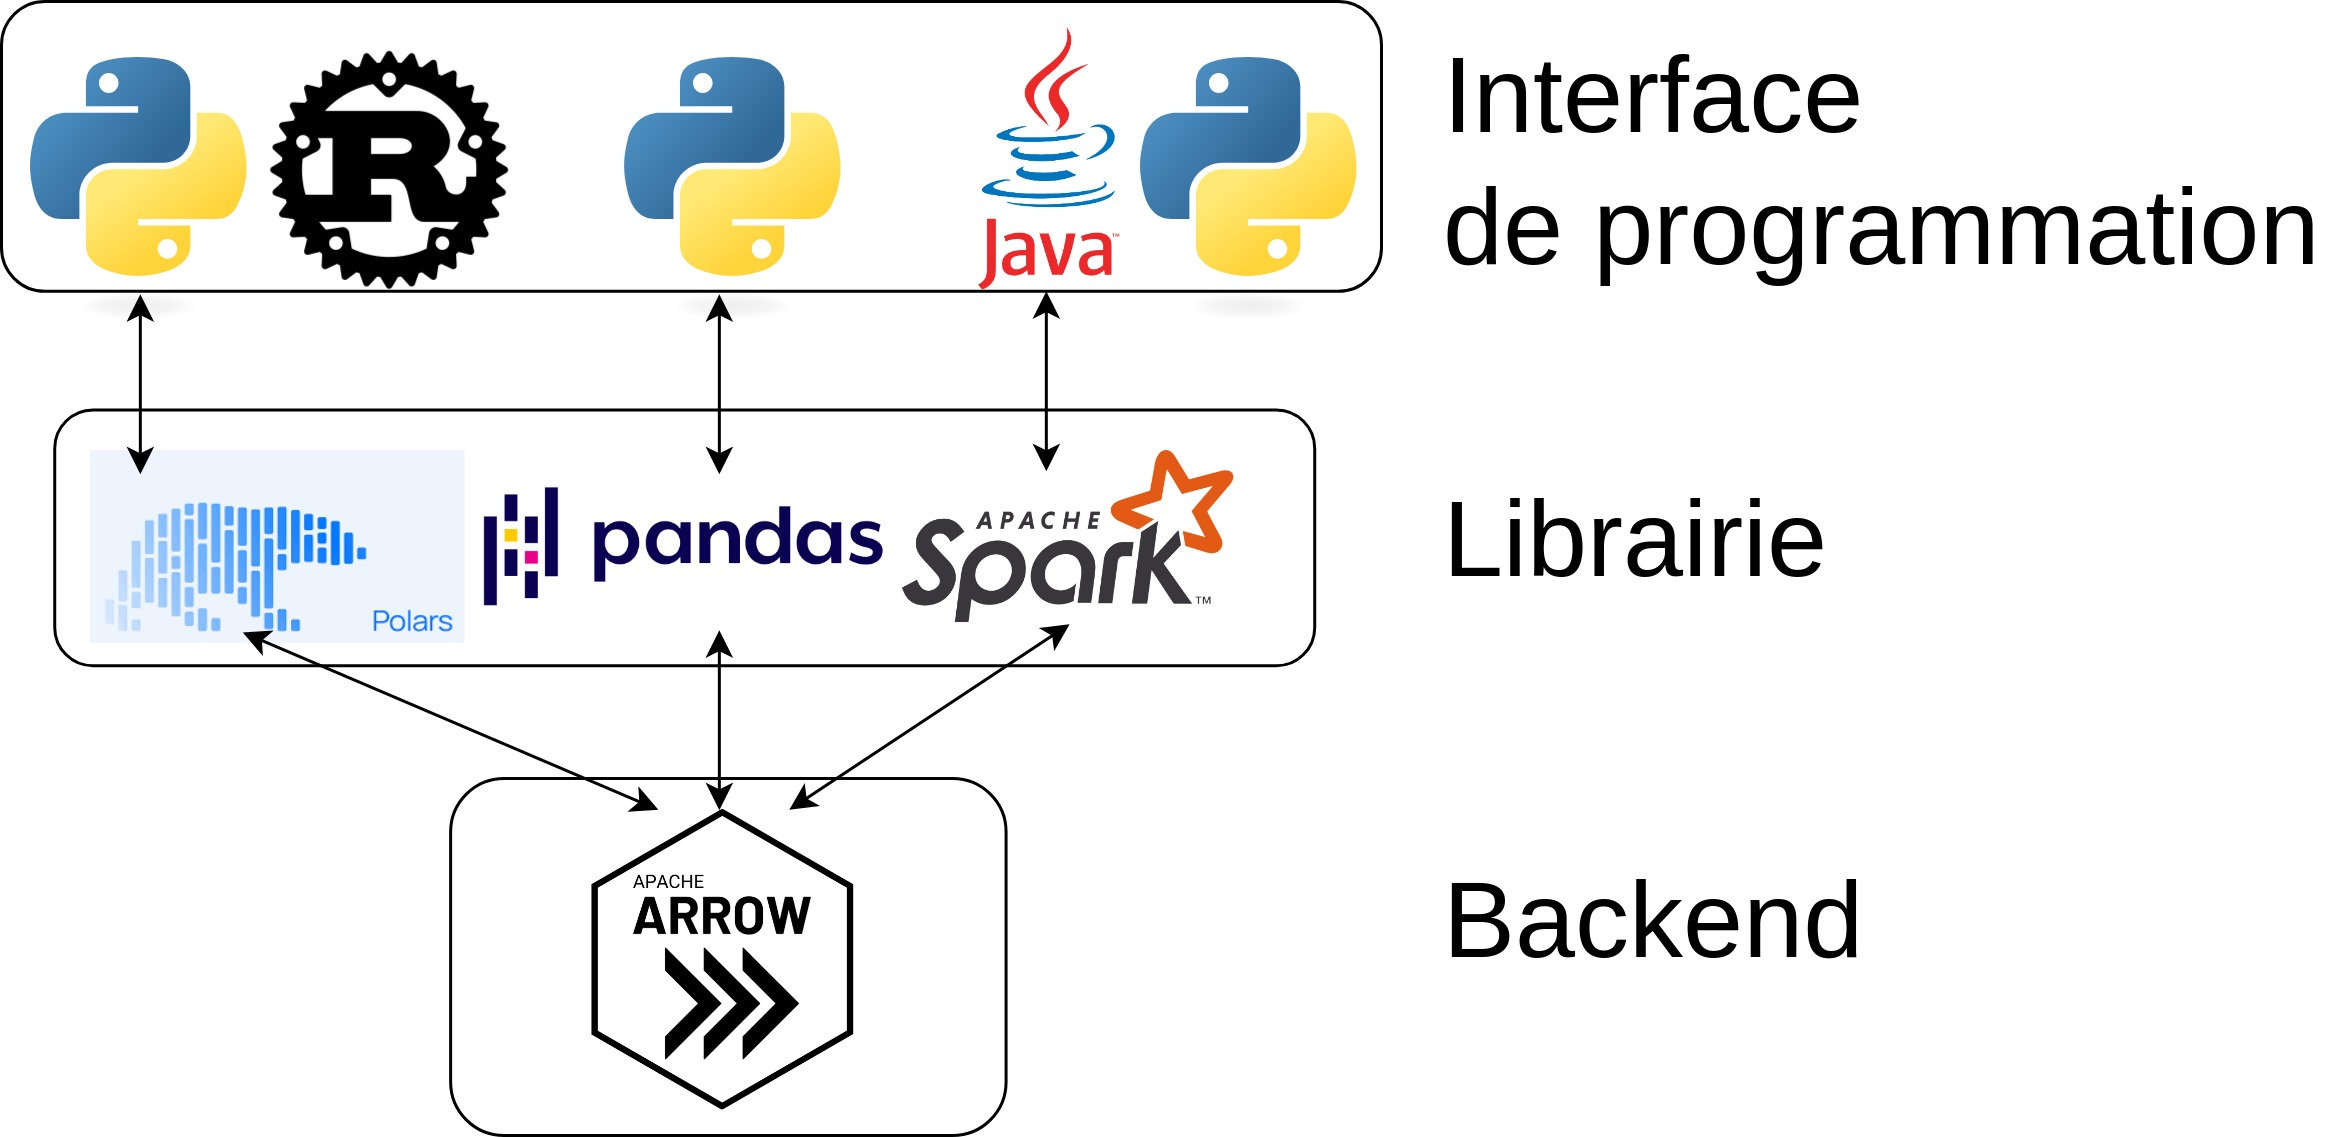
\includegraphics[width=11cm]{image/from-backend-to-language}
    \end{frame}

    \begin{frame}{Librairies d'analyse de données}
        Pandas 2, sortie en avril 2023, intègre le support de PyArrow pour les DataFrames.
        Il permet des performances supérieures à celles de NumPy pour de bon nombre de traitements\footnote{Pandas 2.0 vs Pandas 1.3 - Performance Comparison, \url{https://medium.com/@santiagobasulto/pandas-2-0-performance-comparison-3f56b4719f58}}\footnotestep{}\footnote{\label{datacamp-pandas2}Pandas 2.0~: What’s New and Top Tips, \url{https://www.datacamp.com/blog/pandas-2-what-is-new-and-top-tips}}.
        \bigbreak
        \centering
        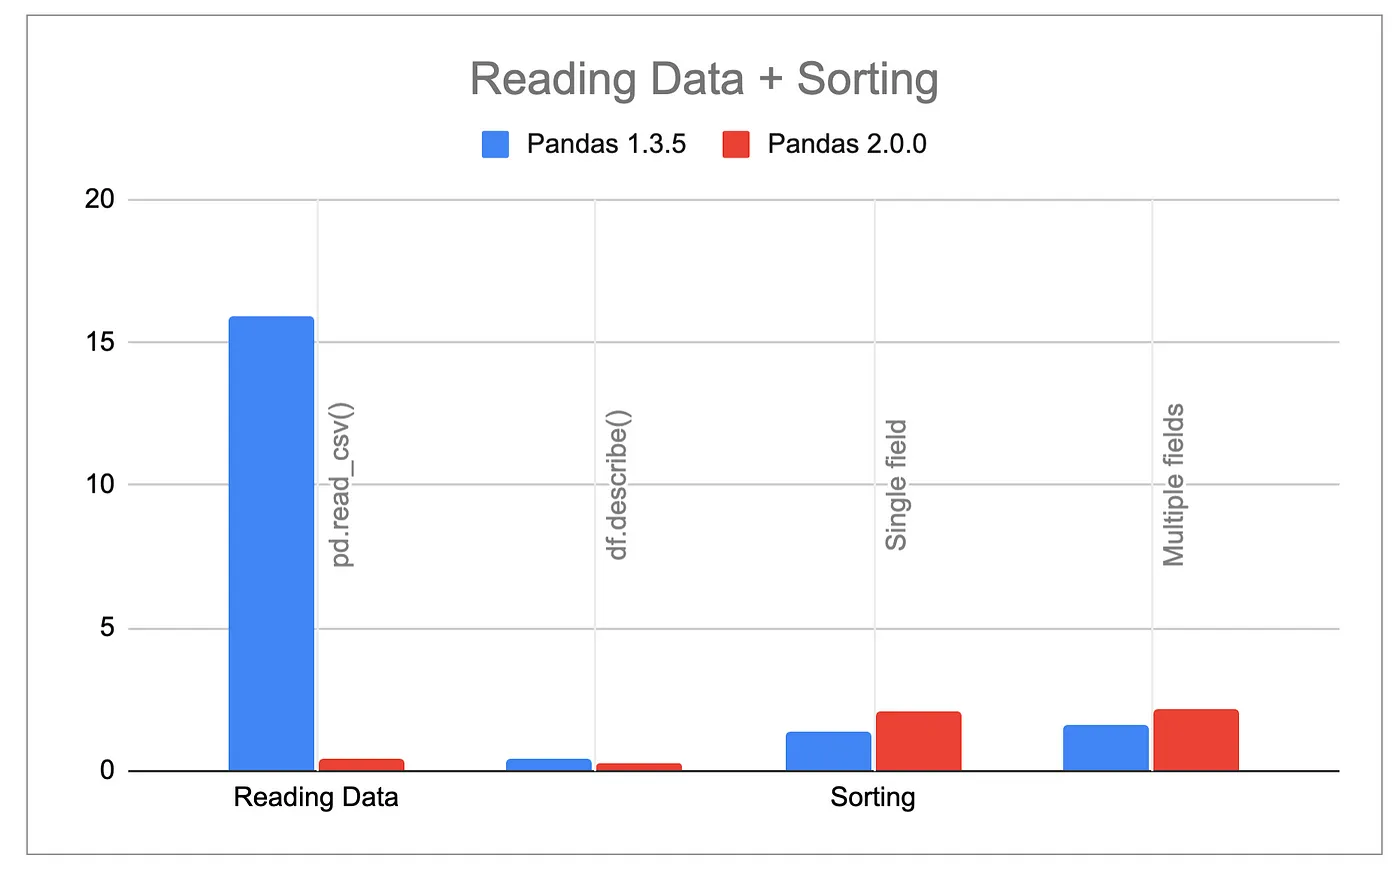
\includegraphics[width=6cm]{image/pandas-1-vs-2}
    \end{frame}

    \begin{frame}{Librairies d'analyse de données}
        La release de Pandas 2 a également pour objectif de ne pas être distancée par Polars/PyPolars, très similaire à Pandas, mais plus performant\cref{datacamp-pandas2}.
        \bigbreak
        \centering
        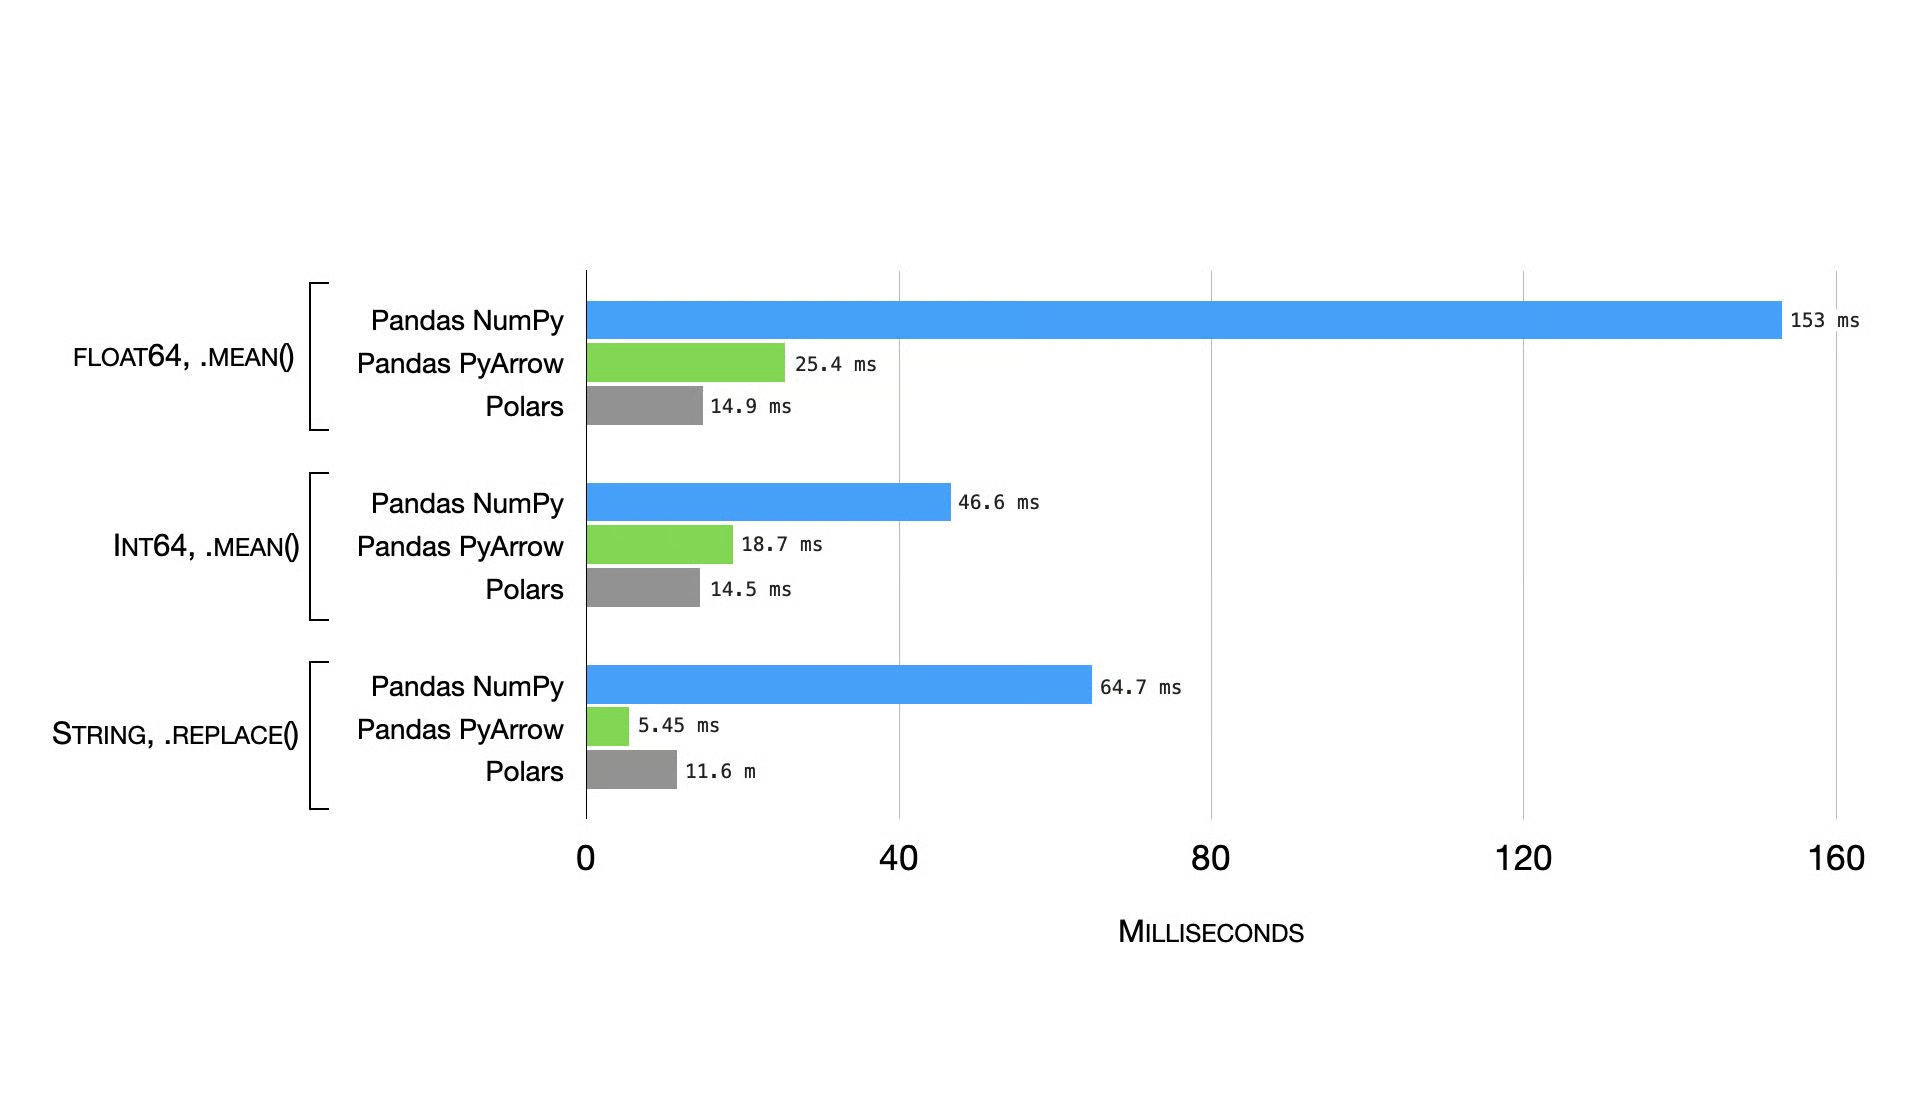
\includegraphics[width=11cm]{image/pandas-numpy-arrrow-polars}
    \end{frame}

    \subsection{Pourquoi Pandas en plus de NumPy et PyArrow~?}

    \begin{frame}{Pourquoi Pandas en plus de NumPy et PyArrow~?}
        \begin{itemize}
            \item Numpy est adapté aux array et non aux données tabulaires
            \item PyArrow est adapté aux données tabulaires mais n'a pas une API Python simple, manque de connecteurs (SQL, Excel, \textit{etc}).
            \item Pandas est adapté aux données tabulaires, a une API Python simple et possède de nombreux connecteurs pour lire et écrire des données dans différents formats (CSV, Excel, SQL, JSON, Parquet, \textit{etc}).
        \end{itemize}
        \bigbreak
        \begin{dangercolorbox}
            Le métier de data scientist n'est pas celui de développeur Python.
            Il est important que les API des outils à sa disposition soit clairs\ldots
        \end{dangercolorbox}
    \end{frame}

    \subsection{Structures de données (Series, DataFrame)}
    \begin{frame}[fragile]{Structures de données (Series, DataFrame)}
        Un \lstinline{DataFrame} est une structure de données tabulaire, similaire à une feuille de calcul Excel ou une table SQL.

        Une \lstinline{Serie} est l'équivalent d'une colonne dans un \lstinline{DataFrame}.
        \begin{lstlisting}[language=bash]
In [47]: car = pd.DataFrame({"model": ["Mercedes", "BMW", "Dacia"], "price": [41_000, 37_000, 15_000]})
In [48]: print("Type of car DataFrame is : ", type(car))
Type of car DataFrame is :  <class 'pandas.core.frame.DataFrame'>
In [49]: print("Type of car price column is : ", type(car["price"]))
Type of car price column is :  <class 'pandas.core.series.Series'>
        \end{lstlisting}
    \end{frame}

    \begin{frame}{Structures de données (Series, DataFrame)}
        \centering
        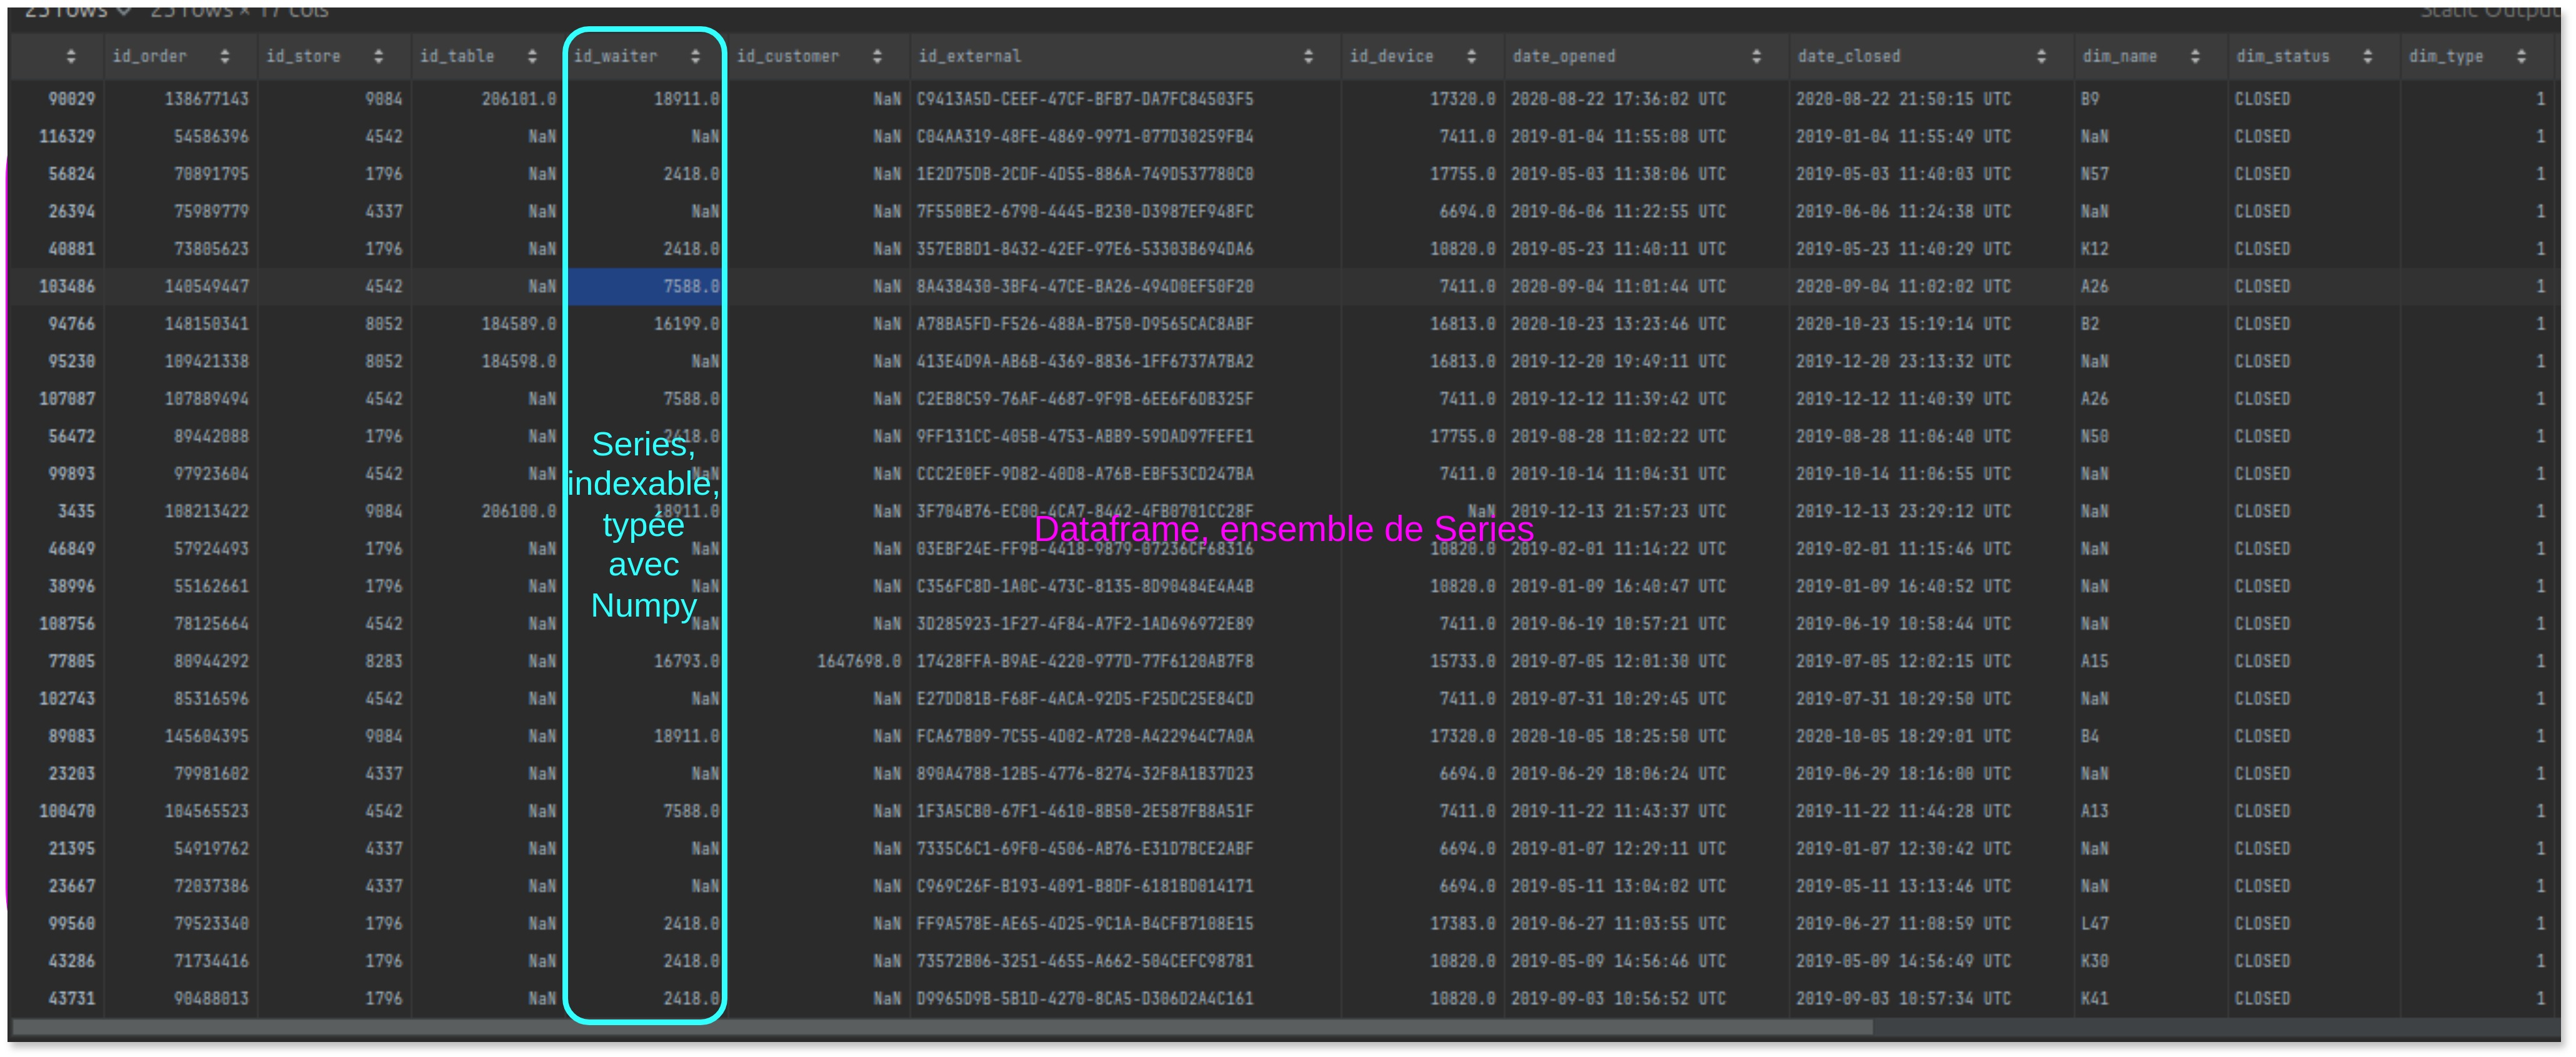
\includegraphics[width=12cm]{image/dataframe-n-series}
    \end{frame}


    \section{Traitement des principaux formats de fichiers}

    \subsection{Excel, CSV, XML, JSON, Parquet, \ldots}
    \begin{frame}{Excel, CSV, XML, JSON, Parquet, \ldots}
        Selon la documentation de Pandas, cette librairie peut lire de nombreux types de fichiers pour en faire des \lstinline{pandas.DataFrame}~:
        \begin{columns}
            \column{0.5\textwidth}
            \begin{itemize}
                \item Des fichiers XML, avec \href{https://pandas.pydata.org/docs/reference/api/pandas.read_xml.html}{\lstinline{pandas.read_xml}}
                \item Des fichiers Parquet, avec \href{https://pandas.pydata.org/docs/reference/api/pandas.read_parquet.html}{\lstinline{pandas.read_parquet}}
                \item Des fichiers Excel, avec \href{https://pandas.pydata.org/docs/reference/api/pandas.read_excel.html}{\lstinline{pandas.read_excel}}
                \item Des fichiers CSV, avec \href{https://pandas.pydata.org/docs/reference/api/pandas.read_csv.html}{\lstinline{pandas.read_csv}}
                \item Des fichiers JSON, avec \href{https://pandas.pydata.org/docs/reference/api/pandas.read_json.html}{\lstinline{pandas.read_json}}
            \end{itemize}
            \column{0.5\textwidth}
            \centering
            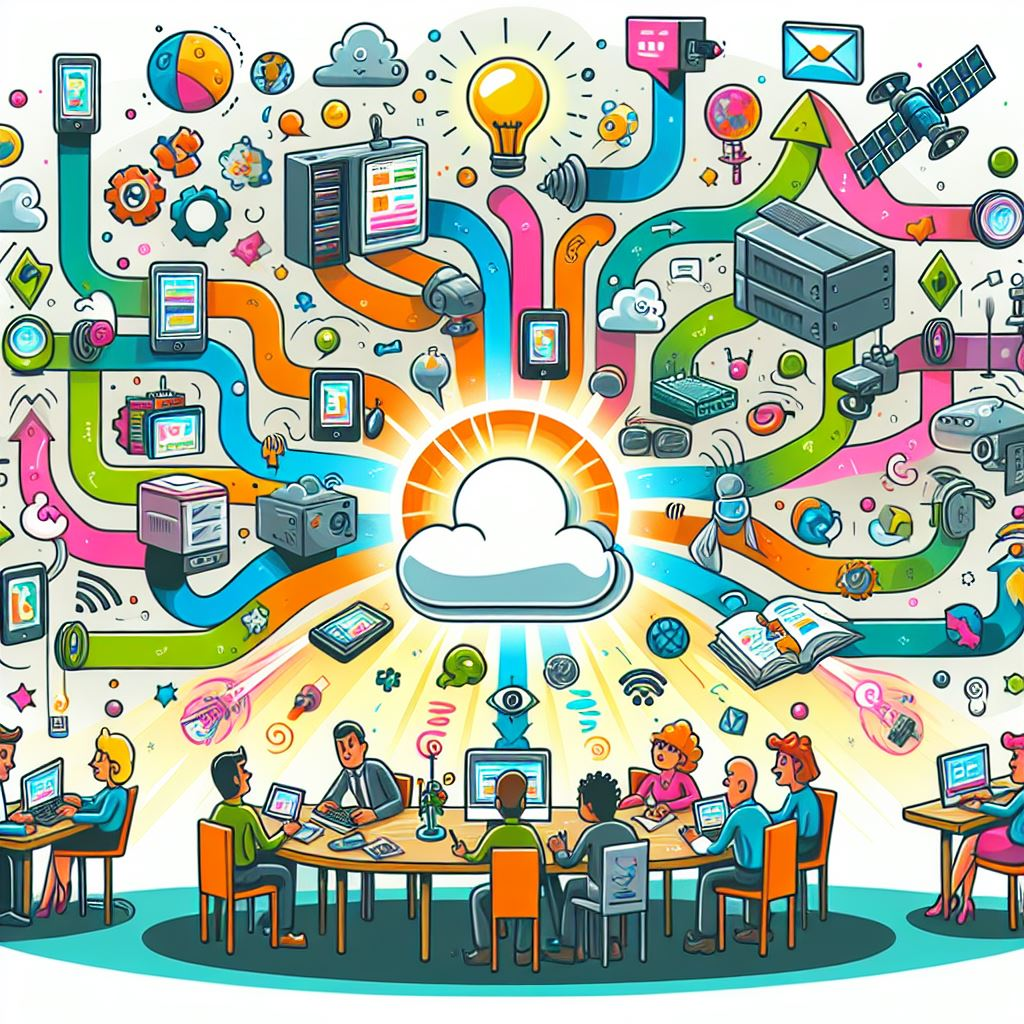
\includegraphics[width=7cm]{image/data-from-everywhere}
        \end{columns}
    \end{frame}

    \subsection{Requêtes SQL avec Pandas}
    \begin{frame}{Requêtes SQL avec Pandas}
        Pandas est compatible avec tous les moteurs de bases de données SQL.
        \begin{itemize}
            \item La méthode \href{https://pandas.pydata.org/docs/reference/api/pandas.read_sql.html}{\lstinline{pandas.read_sql}} permet de lire des données depuis une base de données SQL et de les convertir en \lstinline{pandas.DataFrame} avec une requête SQL classique.
            \begin{dangercolorbox}
                Elle nécessite le connecteur/driver client correspond au moteur de base de données, \lstinline{mysql-connector-python} pour MySQL.
            \end{dangercolorbox}
            \item La méthode \href{https://pandas.pydata.org/docs/reference/api/pandas.DataFrame.to_sql.html}{\lstinline{pandas.DataFrame.to_sql}} permet d'écrire un \lstinline{pandas.DataFrame} dans une table d'une base de données SQL.
            \begin{dangercolorbox}
                Elle nécessite SQLAlchemy ou \lstinline{sqlite3.Connection} pour se connecter à la base de données.
            \end{dangercolorbox}
        \end{itemize}
    \end{frame}

    \subsection{Localiser des données avec les masques}
    \begin{frame}[fragile]{Localiser des données avec les masques}
        Un masque est un tableau de booléens qui permet de filtrer les données d'un \lstinline{pandas.DataFrame} ou d'une \lstinline{pandas.Series}.
        Il est utilisé pour sélectionner les lignes ou les colonnes qui répondent à une condition.
        \bigbreak
        \begin{lstlisting}[language=python]
df_7965 = df_orders[df_orders["id_store"] == 7965]
        \end{lstlisting}
        \begin{dangercolorbox}
            Appliquer le tableau ne modifie le DataFrame, il permet d'en retourner un nouveau qui faut assigner à une nouvelle variable.

            Il en va de même pour la plupart des transformations de DataFrame, elle ne sont pas \textit{in place} il faut penser à stocker le retour.
            Certaines exceptions cependant, comme \lstinline{pandas.DataFrame.drop} qui modifie le DataFrame en place si l'on change la valeur de l'argument inplace à True.
        \end{dangercolorbox}
    \end{frame}


    \section{Préparation et nettoyage des données}

    \subsection{Traitement des données manquantes}

    \begin{frame}[fragile]{Traitement des données manquantes}
        Des données manquantes peuvent bloquer l'insertion en base SQL de données.
        En cas de schéma \lstinline{NOT NULL} par exemple.
        \bigbreak
        Plusieurs options sont possibles pour traitement ce manque de données.
        \begin{itemize}
            \item Supprimer la ligne ou la colonne contenant des données manquantes.
            \item Remplacer les données manquantes par une valeur par défaut, comme 0, la moyenne, la médiane, le mode, \textit{etc}.
            \item Utiliser des techniques de machine learning pour prédire les valeurs manquantes en fonction des autres données.
        \end{itemize}
        \bigbreak
        \begin{lstlisting}[language=python]
df_sub_mask = df_sub["id_store"] == 4542
df_sub_filtered = df_sub[df_sub_mask]
assert len(df_sub_filtered["id_store"].notnull()) == len(df_sub[df_sub_mask])
        \end{lstlisting}
        Les méthodes \lstinline{pandas.DataFrame.dropna} et \lstinline{pandas.DataFrame.fillna} permettent de supprimer ou de remplacer les données à NA/NaN.
        \lstinline{pandas.DataFrame.notnull} et \lstinline{pandas.DataFrame.isnull} permettent de vérifier si les données sont manquantes ou non.
    \end{frame}

    \begin{frame}{Traitement des données manquantes}
        \begin{columns}
            \column{0.5\textwidth}
            \centering
            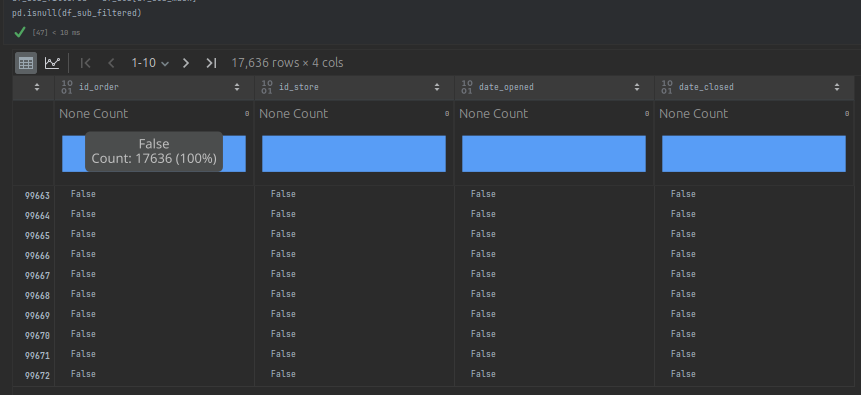
\includegraphics[width=6cm]{image/pandas-isnull}
            \column{0.5\textwidth}
            \centering
            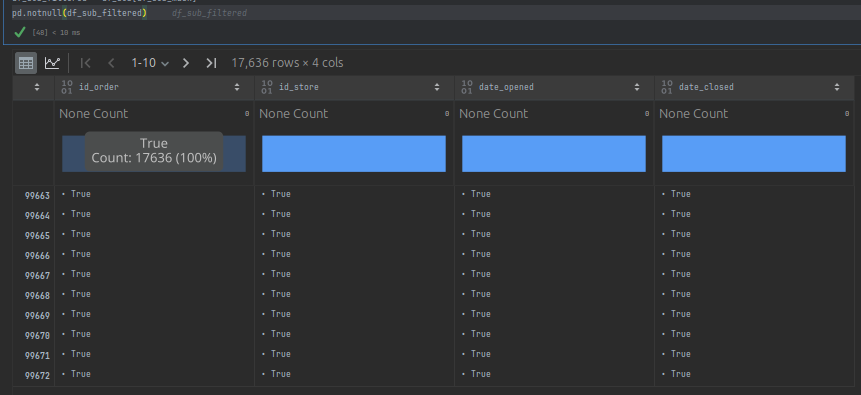
\includegraphics[width=6cm]{image/pandas-notnull}
        \end{columns}
    \end{frame}

    \subsection{YData Profiling}
    \begin{frame}{YData Profiling}
        Librairie qui permet de générer un rapport d'analyse exploratoire des données d'un \lstinline{pandas.DataFrame} en une ligne.
        \bigbreak
        Il permet entre autre~:
        \begin{itemize}
            \item de visualiser les données manquantes
            \item de visualiser les distributions des variables, comme un \lstinline{pandas.DataFrame.describe}
            \item de visualiser les corrélations entre les variables
            \item de visualiser les valeurs aberrantes
            \item Many more\ldots{}
        \end{itemize}
        Cette librairie permet de savoir facilement quelles données sont à néttoyer, supprimer.
    \end{frame}

    \subsection{Combinaison et transformation de données}

    \subsection{Agrégation et regroupement de données}

    \begin{frame}
        Si il y a une colonne en trop
    \end{frame}

    \subsection{Traitement des données temporelles}


    \section{Les types en Numpy et Pandas}

    \subsection{Les types en Numpy}\label{numpy-typing}

    \begin{frame}[fragile]{Les types en Numpy et Pandas}{Numpy}
        On dit que les types sont \textit{inférés}~:
        \begin{lstlisting}[language=bash]
Out[5]: import numpy as np
np.array([1, 2, 3, True])
Out[6]: array([1, 2, 3, 1])
np.array([1, 2, 3, "4"])
Out[7]: array(['1', '2', '3', '4'], dtype='<U21')
np.array([1, 2, 3, "4444444444555555555555555555555555"])
Out[8]: array(['1', '2', '3', '4444444444555555555555555555555555'], dtype='<U34')
        \end{lstlisting}
        Qu'observe-t-on~?
        \pause
        \bigbreak
        Numpy trouve le plus petit (en termes de taille mémoire) type commun à tous les éléments du tableau.
    \end{frame}

    \subsection{Les types en Pandas}\label{pandas-typing}
    \begin{frame}[fragile]{Les types en Numpy et Pandas}{Pandas}
        De même les types sont \textit{inférés}~:
        \begin{lstlisting}[language=bash,basicstyle=\tiny\ttfamily]
import pandas as pd
pd.DataFrame({"model": ["Mercedes", "BMW", "Dacia"], "price": [41_000, 37_000, 15_000]})
Out[20]:
      model  price
0  Mercedes  41000
1       BMW  37000
2     Dacia  15000
pd.DataFrame({"model": ["Mercedes", "BMW", "Dacia"], "price": [41_000, 37_000, "15_000"]}).info()
<class 'pandas.core.frame.DataFrame'>
RangeIndex: 3 entries, 0 to 2
Data columns (total 2 columns):
 #   Column  Non-Null Count  Dtype
---  ------  --------------  -----
 0   model   3 non-null      object
 1   price   3 non-null      object
dtypes: object(2)
memory usage: 180.0+ bytes
        \end{lstlisting}
        Qu'observe-t-on~?
        \pause
        \bigbreak
        Numpy trouve le plus petit (en termes de taille mémoire) type commun à tous les éléments du tableau.
    \end{frame}

    \begin{frame}[fragile]{Les types en Numpy et Pandas}{Pandas}
        Peut-on mieux faire~?
        \pause
        \bigbreak
        Oui, Pandas par sécurité, pour ne pas perdre d'information, utilise des entiers 64 bits.
        Inutiles ici, car un 16 bits car un 16 bits non signé va jusqu'à 65 535, attention avec une Ferrari\ldots
        \begin{lstlisting}[language=bash,basicstyle=\tiny\ttfamily]
car = pd.DataFrame({"model": ["Mercedes", "BMW", "Dacia"], "price": [41_000, 37_000, 15_000]})
car = car.astype({"model": pd.StringDtype(), "price": pd.UInt16Dtype()})
car.info()
<class 'pandas.core.frame.DataFrame'>
RangeIndex: 3 entries, 0 to 2
Data columns (total 2 columns):
 #   Column  Non-Null Count  Dtype
---  ------  --------------  -----
 0   model   3 non-null      string
 1   price   3 non-null      UInt16
dtypes: UInt16(1), string(1)
memory usage: 165.0 bytes
car.head()
Out[44]:
      model  price
0  Mercedes  41000
1       BMW  37000
2     Dacia  15000
pd.UInt16Dtype.type # C'est en fait un type Numpy
Out[45]: numpy.uint16
        \end{lstlisting}
    \end{frame}

    \subsection{Exercice}\label{pandas-exercice}
    \begin{frame}{Pandas}{Exercice \execcounterdispinc{}}
        Ouvrir le Notebook \url{https://github.com/DigicompClassesByPapIT/PYDATA/blob/main/3_pandas.ipynb}.
        \bigbreak
        \centering
        
\includegraphics[width=7cm]{image/digicomp-lightbulb}
    \end{frame}


    \section{Visualisation avec Plotly}

    \subsection{Types de graphiques~: ligne, point, histogramme, bar, pie, ...}

    \subsection{Label, légende, grille, axes, titre}


    \section{Exemple d'analyse de données financières}


    \section{Introduction au Machine Learning}\label{sec:ml}
    \begin{frame}{Introduction au Machine Learning}{Les librairies}
        Python est le langage de la Data Science et du Machine Learning.
        Il surpasse depuis des années l'écosystème \href{https://posit.co/download/rstudio-desktop/}{R}.
        \bigbreak
        Mais la Data Science nécessite de nombreuses librairies, les plus connues sont~:
        \begin{itemize}
            \item \href{https://numpy.org/}{NumPy} pour les calculs scientifiques
            \item \href{https://pandas.pydata.org/}{Pandas} pour la manipulation de données
            \item \href{https://matplotlib.org/}{Matplotlib} pour la visualisation de données
            \item \href{https://plotly.com/}{Plotly} pour la visualisation de données
            \item \href{https://scikit-learn.org/stable/}{Scikit-learn} pour le Machine Learning
            \item \href{https://www.tensorflow.org/}{TensorFlow} pour le Deep Learning
            \item \href{https://pytorch.org/}{PyTorch} pour le Deep Learning
        \end{itemize}
    \end{frame}

    \begin{frame}{Introduction au Machine Learning}{Régression linéaire avec Scikit-learn}
        Télécharger et ouvrir le notebook \url{https://github.com/DigicompClassesByPapIT/Python/blob/main/15_simple_linear_regression}.
        Ce dernier illustre un exemple de régression linéaire simple avec Scikit-learn.
        \bigbreak
        \begin{columns}
            \column{0.5\textwidth}
            La regression linéaire est un des plus simples algorithmes de Machine Learning.
            Il permet de prédire une variable continue à partir d'une autre variable continue en trouvant la meilleure droite qui les relie.
            Celle qui a le R carré le plus élevé, le plus proche de 1.
            \column{0.5\textwidth}
            \centering
            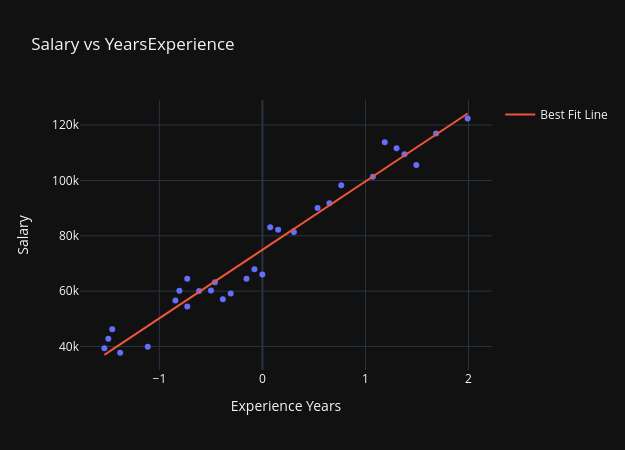
\includegraphics[width=6cm]{image/linear-regression}
        \end{columns}
        \bigbreak
        Le salaire est la variable \textit{target} qui pourra être prédite à partir de l'expérience la variable année d'expérience, la \textit{feature}.
    \end{frame}

    \begin{frame}{Introduction au Machine Learning}{Régression linéaire avec Scikit-learn}
        Avec la méthode \lstinline{train_test_split} de Scikit-learn on peut diviser les données en deux jeux~:
        \begin{itemize}
            \item Un jeu d'entraînement pour entraîner le modèle et trouver la meilleure regression linéaire
            \item Un jeu de test pour tester le modèle et calculer le R carré et d'autres métriques, sur un jeu de données inconnues.
        \end{itemize}
        \begin{dangercolorbox}
            Le Machine Learning n'est qu'un domaine de la Data Science.
            Il a besoin des mêmes outils pour le pré-traitement des données (A.K.A \textit{data wrangling}), la visualisation, la manipulation, \textit{etc}.
            Pour ce faire il faut maîtriser les librairies \lstinline{pandas}, \lstinline{plotly}.
            \lstinline{pandas} est une librairie très puissante pour la manipulation de données, elle est très utilisée en Data Science.
            Elle n'est pas compliquée mais mériterait une journée de formation à elle seule.
            Regardez les notebook \url{https://github.com/jupyter-naas/awesome-notebooks/tree/master/Pandas} pour vous autoformer.
        \end{dangercolorbox}
    \end{frame}

    \begin{frame}{Introduction au Machine Learning}{Régression linéaire avec Scikit-learn}
        Exercice \execcounterdispinc{}, créer un notebook et étudier le dataset \url{https://github.com/DigicompClassesByPapIT/PYDATA/blob/main/advertising.csv}.
        Il contient les données de ventes en fonction de la publicité TV, radio et journaux.
        \bigbreak
        La variable \textit{target} est les ventes, les \textit{features} sont les budgets publicitaires.
        Trouver quelle est la meilleure \textit{feature} de prédiction des ventes, celle qui a le R carré le plus élevé.
    \end{frame}


    \section{Licence CC}\label{sec:licence}

    \begin{frame}{Licence}{Licence Creative Commons}
        Support de cours sous licence Creative Commons BY-NC-ND~.
        \bigbreak
        Vous pouvez donc, partager, copier, distribuer le document.
        \bigbreak
        Attribution requise à PapIT SASU - Pas d’utilisation commerciale - Pas de modification
        \bigbreak
        \centering
        
\includegraphics[width=5cm]{image/by-nc-nd-logo}
    \end{frame}

\end{document}
